\documentclass{algo-paper}

%\usepackage{algo-paper}
%\documentclass[a4paper, oneside]{scrartcl}

% Zeichensatz und Sprachpaket
\usepackage[ngerman]{babel} 
\usepackage{arev}

% Einrücken eines neues Absatzes auf 0
\parindent 0pt
\parskip 6pt
%\usepackage{titlesec}
%\titlespacing{\section}{0pt}{1em}{0.3em}
\setcounter{secnumdepth}{3}

% Unterpunkte in Aufzählungen andere Symbole geben
%\usepackage{pifont}
%\renewcommand{\labelitemi}{\ding{104}}
%\renewcommand{\labelitemii}{\ding{105}}
\renewcommand*\labelitemii{$\circ$}
%\renewcommand{\thesection}{\Alph{section}} 

%\usepackage{tabularx}

% Abstand zwischen Aufzählungen kleiner definieren 
%\let\origitemize\itemize	
%\def\itemize{\origitemize\itemsep0pt}

% Für TODOs
\usepackage{todonotes}

% Quellen Einstellung
%\bibliographystyle{IEEEtranSA}	% english style

% Algorithmen
\usepackage[german, linesnumbered]{algorithm2e}

%Dokument Info
\title{Kräftebasierter Layoutalgorithmus für hierarchische Argumentkarten}
\subtitle{\vskip 2.5em Seminararbeit zur Veranstalltung Visualisierung komplexer Argumentation \vskip 1.5em}
\author{Christian, Jonathan, Sven, Michael, Sebastian, Mira}
\publishers{
\normalfont\normalsize Betreut durch: \\[0.5\baselineskip]

\normalfont\large Jun.-Prof. Gregor Betz, Diplom Inform. Andreas Gemsa und Dr. Ignaz Rutter
}
\date{}


% Formelzeugs
\usepackage{amsfonts}   
\usepackage{amssymb}
\usepackage{amsmath}
\def\L{\ensuremath{\mathcal{L}}}
\def\R{\ensuremath{\mathbb{R}}}
\def\RR{\ensuremath{\mathcal{R}}}
\def\C{\ensuremath{\mathbb{C}}}
\def\CC{\ensuremath{\mathcal{C}}}
\def\Z{\ensuremath{\mathbb{Z}}}
\def\N{\ensuremath{\mathbb{N}}}
\def\F{\ensuremath{\mathbb{F}}}
\def\dann{\ensuremath{\Rightarrow}}
\def\gdw{\ensuremath{\Leftrightarrow}}
\def\tr{\ensuremath{\text{tr}}}
\def\deg{\ensuremath{\text{deg}}}
\def\Aut{\ensuremath{\text{Aut}}}
\def\Abb{\ensuremath{\text{Abb}}}

\usepackage[hyperref]{ntheorem}
\theorembodyfont{\normalfont}
\theoremstyle{changebreak} 
\newtheorem{theorem}{Theorem}
\newtheorem{lemma}{Lemma}
\newtheorem*{defi}{Definition}
\newtheorem*{problem}{Problem}

\newcommand{\blankpage}{\clearpage\mbox{}\clearpage}

\usepackage{hyperref}
\renewcommand{\L}{\ensuremath{\mathcal{L}}}

\addto\extrasngerman{%
\def\AMSautorefname{Gleichung}%
\def\Hfootnoteautorefname{Fußnote}%
\def\Itemautorefname{Listenpunkt}%
\def\algocflineautorefname{Algorithmus}%
\def\appendixautorefname{Anhang}%
\def\chapterautorefname{Kapitel}%
\def\definitionautorefname{Definition}%
\def\equationautorefname{Gleichung}%
\def\tableautorefname{Tabelle}%
\def\figureautorefname{Abbildung}%
\def\listingautorefname{Quelltextauszug}%
\def\paragraphautorefname{Absatz}%
\def\partautorefname{Teil}%
\def\sectionautorefname{Abschnitt}%
\def\subfigureautorefname{Abbildung}%
\def\subsectionautorefname{Abschnitt}%
\def\subsubsectionautorefname{Abschnitt}%
\def\theoremautorefname{Theorem}%
}%


\nonfrenchspacing

\makeindex

\begin{document}  


\maketitle
%\begin{titlepage}
\author{Christian, Jonathan, Sven, Michael, Sebastian, Mira}
\date{\today}

% Inhaltabhängig! 
\title{\vspace{3cm}Kräftebasierter Layoutalgorithmus für hierarchische Argumentkarten}
\maketitle
\end{titlepage}

\pagenumbering{roman}
\cleardoublepage



\listoftodos
\cleardoublepage

\pagenumbering{roman}

%\setcounter{tocdepth}{3}
\tableofcontents
%\clearpage
%\pagestyle{empty}
\cleardoublepage

\pagenumbering{arabic}

\chapter{Motivation}
% Was sind Argumentkarten? Wer verwendet sie und wofür?
% Darstellung von Argumentkarten
% - Wie werden sie bis jetzt dargestellt?
% - Wieso will man sie darstellen?
Diese Arbeit beschäftigt sich mit Argumentkarten, manchmal auch Argumentationskarten genannt. Diese dienen als graphische Darstellung von Debatten. Eine Argumentkarte ist die Darstellung einer Debatte in Form eines Graphen.
Auf einer solchen Karte werden die Thesen und Argumente der Debatte als einzelstehende Elemente herausgestellt. 
Zusätzlich lassen sich auf solche einer Karte Beziehungen zwischen Argumenten, welche von unterstützenden oder angreifender Natur sein können, visualisieren.
In \autoref{f:Beispielargumentkarte} ist eine kleine Beispielargumentkarte dargestellt. 
Eine größe Argumentkarte und sowie ein Buch, welches solche enthält, existieren zum Beispiel von Betz und Cacean\cite{ClimateEngineering, betz2012ethical}.


%Debatten werden in der Regel in sogenannten Argumentkarten, manchmal auch Argumentationskarten, dargestellt. 
%Auf einer solchen Karte werden die Thesen und Schlüsse der Debatte in einzelne Sätze aufgeschlossen. Diese Sätze werden dann in einem Graphen abgebildet. 

% Spezielle Anforderungen
% - Wieso Gruppen?
% - Wieso Layout beibehalten? -> Mentale Karte
Die Argumentkarten sind vor allem ein Werkzeug zum besseren Verständnis der Debatte. 
Über die Visualisierung der Elemente und ihre Beziehungen hinaus, existieren weitere Möglichkeiten um das Verstehen der Debatte zu verbessern und zu erleichtern.
So können beispielsweise thematisch verwandte Knoten gruppiert werden. 
Es besteht außerdem die Möglichkeit, Gruppen geschlossen zu visualisieren, also in ihr enthaltene Argumente und Untergruppen nicht anzuzeigen, sondern nur durch ein
Element und den Gruppentitel zu repräsentieren. So kann ein schnellerer  Überblick über die Debatte ermöglichen werden.
Das Hervorheben einzelner Argumentationsstrukturen durch die Wahl des Layouts ist eine weiterer wichtiger Aspekt bei der Visualisierung von Debatten.
%Dabei können verschiedene Aspekte der Debatte in den Vordergrund gerückt werden um diesen besser zu verstehen. 
%Beispielsweise können thematisch verwandte Knoten Gruppiert werden um einen besseren überblick über die Debatte zu ermöglichen 
%oder es können einzelne Arugmentationsstränge besonders hervorgehoben werden.

\begin{figure}[h]
\begin{center}
	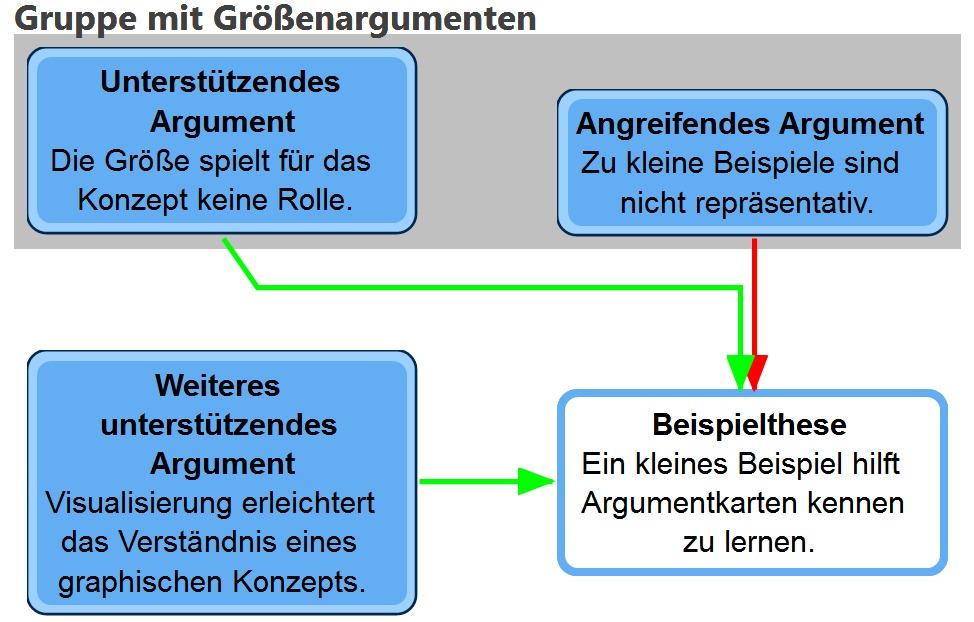
\includegraphics[width=0.5\textwidth]{Pics/Beispielargumentkarte.png}
	\caption{Beispielhafte Argumentkarte mit einer These, drei Argumenten, zwei davon unterstützend und eine angreifend, sowie einer Gruppe.}
	\label{f:Beispielargumentkarte}
\end{center}
\end{figure}

Damit sich die von einer Argumentkarte bereitgestellten Informationen sinnvoll verwenden lassen, muss die Argumentkarte folglich auf eine geeignete Weise dargestellt werden.
Es existieren bereits einige Werkzeuge mit denen Argumentkarten angelegt  und ein Layout automatisch erzeugt werden kann. 
Allerdings müssen die resultierenden Layouts der Argumentkarten oftmals von Hand nachbearbeitet werden, um eine befriedigende Darstellung der Strukturen zu erhalten.
Darüber hinaus ist eine Unterstützung von Gruppen nicht immer gegeben.

% Wie ist diese Ausarbeitung aufgebaut?
%\subsection{Gliederung}
% 1. Problemstellung und -definition
% 2. Lösungsvorschlag
% 3. Detaillierte Erklärung des Algorithmus
% 4. Vergleich zu anderen Lösungsansätzen
In dieser Arbeit geht es um die automatisierte Darstellung von Argumentkarten mit Gruppen, sowie die Interaktion mit diesen Gruppen. 
%und damit um eine Möglichkeit die Argumentkarte zu vereinfachen um dem Benutzer einen schnellen und guten Überblick über die Debatte zu ermöglichen.
Es geht also um die Frage, wie sich Gruppen und Gruppenhierarchien den Anforderungen an Argumentkarten entsprechend visualisieren lassen 
und wie das Layout auf das Öffnen und Schließen von Gruppen reagiert.
%\todo[inline]{Lösungsanstz in Kurzform}

Im nächsten \autoref{chapter:layoutproblem}  präzisieren und abstrahieren wir diese Problemstellung. 
In \autoref{chapter:algo} präsentieren wir unseren Lösungsansatz, welchen wir dann in \autoref{chapter:vgl} mit alternativen Ansätzen vergleichen und bewerten.
\autoref{ch:zsf} schließt mit einer Zusammenfassung.

%-----------------------------------------------------------------------------------------------------------------------------------------------------------------------------------
\chapter{Problemstellung}%\chapter{Layoutproblem} % > mehr als Layout, betrachte auch Interaktion!
\label{chapter:layoutproblem}
In diesem Kapitel definieren wir das von uns behandelte Layoutproblem für Argumentkarten mit Gruppenstruktur, sowie die Anforderungen für Interaktionen mit dem Layout.
Wir beschreiben also wie ein das Layout aussehen soll und was beim Öffnen und Schließen einer Gruppe beachtet werden muss.

\section{Layoutproblem}
\label{sec:layoutproblem}
% Was ist das grundlegende Problem? -> Layout finden
Das Zeichnen eines Graphen setzt sich aus dem Finden eines Layouts sowie des Renders zusammen. 
Für uns von Interesse ist nur ersteres, das Layoutproblem. 
Ziel hierbei ist es für einen gegebenen Graphen und gegebenenfalls weitere Informationen algorithmisch ein Layout zu berechnen,
welches gewisse Zeichenkonventionen erfüllt, erwünschte Ästhetikkriteren optimiert und gegebenenfalls weiteren lokalen Nebenbedingungen genügt.

% Was macht das Problem speziell? -> Gruppen und dass für Argumentkarten
% Was lässt sich jedoch abstrahieren? -> knoteninhalt, kanten
Im Fall der Argumentkarten abstrahieren wir für das Layoutproblem einige Informationen. 
So spielen die Texte der einzelnen These oder Argumente für uns keine Rolle. 
Sie werden lediglich durch achsenparallele Rechtecke als Knoten des Graphen repräsentiert.
Des Weiteren ignorieren wir bei den Beziehungen zwischen Elementen den Typ sowie die Richtung. 
Es ist also lediglich von Relevanz ob zwei Elemente in einer Beziehung stehen.
Dies wird dann durch eine ungerichtete Kante repräsentiert. 
Eine geschlossene Gruppe wird als Pseudoknoten aufgefasst und durch ein leeres Element repräsentiert.
Dies kann  z.B. ein Rechteck oder ein Kreis sein.  Die Kindgruppen und Knoten einer geschlossenen Gruppe sind folglich verborgen.
Falls auch offene Gruppe dargestellt werden, sollten diese ihre Kindknoten umfassen. 
In einem in \autoref{chapter:vgl} alternativen Ansatz werden offenen Gruppen nicht explizit dargestellt.

Die Eingabe des Algorithmus lässt sich mit diesen Abstraktionen formal beschreiben. Sie setzt sich als aus einem Graphen $G=(V,E)$, sowie einem Baum $T$, genannt Gruppenbaum,  und einem Schnitt $S$ durch $T$, welcher die Gruppen sowie deren Zustand repräsentieren.
Die Wurzel $r$ der Baumstruktur repräsentiert die ganze Karte, jeder Knoten aus $V$ ist ein Blatt in $T$ und jeder innere Knoten steht für eine Gruppe.
Durch die Distanz eines inneren Knotens zur Wurzel weißen wir die Gruppen einzelnen Stufen zu. Da Bäume in der Regel auf dem Kopf gezeichnet werden, bezeichne
eine niedrigere Stufe eine höhere Distanz zur Wurzel. Die oberste Stufe sei die Stufe der Wurzel.
Für den Schnitt $S$ von $T$ ist gefordert, dass er jeden Pfad von einem Blatt zur Wurzel genau einmal schneidet.
Ein Knoten wird nur angezeigt, wenn der Schnitt den Pfad zur Wurzel von diesem Knoten in der zu diesem Knoten adjazenten Kante schneidet. 
In anderen Worten also direkt über dem Knoten.
Eine Gruppe wird geschlossen, also als Pseudoknoten, dargestellt, wenn der Pfad zur Wurzel in der adjazenten Kante geschnitten wird und offen, wenn der Pfad zur Wurzel nicht geschnitten wird. In allen anderen Fällen sind die Knoten oder Gruppen hinter einer geschlossenen Gruppe verborgen und werden nicht angezeigt.

%Unter Einbeziehung von Gruppen kann die Eingabe des Algorithmus dann in der Form $G = (V,V_g,E,\sigma)$ dargestellt werden. 
%Die Mengen und Abbildungen dieses Graphen werden im folgenden Beschrieben:
%\todo[inline]{Baumstruktur, Schnitt}
%\todo[inline]{Bulletpoints entfernen}
%\begin{itemize}
%	\item Knoten $V$, Knoten die eine Aussage repräsentieren.
%	\item Gruppenknoten $V_g$, Knoten die eine Gruppe repräsentieren.
%	\item Kanten $E \subseteq \bar{V} \times \bar{V}$, wobei $\bar{V}$ die Menge aller Knoten ($\bar{V} = V \cup V_g$) ist.
%	%\item Rechtseindeutige Abbildung $\lambda(v): V \rightarrow B$, Die Knoten auf die Beschriftungsmenge $B$ (den Text der Knoten) abbildet.
%	 \item Rechtseindeutige Abbildung $\sigma: \bar{V} \rightarrow V_g$, Die Knoten auf ihre Gruppe abbildet (Gruppen können weitere Gruppen enthalten).
%\end{itemize}

\todo[inline]{Beispielgraph/layout (vorziehen) und Baum und Schnitt hinzufügen?}
Für diese Eingabe definieren wir im folgenden die Zeichenkonventionen und die Ästhetikkriterien des Layoutproblems.

%\section{Formale Beschreibung}\label{sec:formaldesc}
%Eine Argumentkarte lässt sich abbilden auf einen beschrifteten gerichteten Graphen.
%Ein solcher Graph $G = (V, E, \lambda_{v}, \lambda_{e})$ mit Knoten $V$, Kanten $E \subseteq V \times V$, Knotenbeschriftungen $\lambda_{v}:V \rightarrow B_v$ und Kantenbeschriftungen $\lambda_{e}: E \rightarrow B_e$. Dabei sind $B_v$ und $B_e$ die Beschriftungsmengen von Knoten bzw. Kanten.
%Auf einen solchen Graphen lässt sich lässt sich eine Argumentkarte Abbilden wenn die Kantenart als Kantenbeschriftung und der Knotentext als Knotenbeschriftung modelliert wird.
%Gegeben einem solchen beschrifteten gerichteten Graphen kann das Layouten eines Graphen als folgendes Problem modelliert werden:
%\begin{description}\item[Eingabe] \hfill \\[0.3\baselineskip]
%			Beschrifteter gerichteter Graph $G = (V, E, \lambda_{v}, \lambda_{e})$ \hfill \\
			% = \{ \text{achsenparallele Rechtecke}\}
			%sowie einen Gruppenzugehörigkeitsbaum 	
%	\item[Ausgabe] \hfill \\[0.3\baselineskip] Zeichnung mit:
%		\begin{itemize}
%		\item $\forall x,y\in V, x \neq y: x \cap y = \emptyset$, also Knoten paarweise disjunkt
%		\item Überschneidungsfreiheit von Knoten: $\forall x, y \in V: x \neq y \Leftrightarrow x \cap y = \emptyset$
%		\item Überlagerungsfreiheit der Kanten: $\forall x, y \in E: x \neq y \Rightarrow \sigma(x, y) \leq 1$. Wobei $\sigma(x, y): E \times E \rightarrow \mathbb{N}_0$ eine Funktion ist, die für zwei Kanten $x$ und $y$ die Anzahl der Schnittpunkte angibt.
				%$\forall x \in V, (y,z) \in E, y\neq x\neq z: x \cap (y,z) = \emptyset$, also Kanten schneiden nur inzidente Knoten
%		\item Sonstige Nebenbedingung (Layoutanforderungen)
%	\end{itemize}\end{description}


\myparagraph{Zeichenkonventionen}
Zeichenkonventionen beschreiben wie Knoten und Kanten gezeichnet beziehungsweise gelayoutet werden sollen. Sie müssen erfüllt werden.
Für das Layoutproblem von Argumentkarten mit Gruppenstruktur sind dies im Einzelnen:
\begin{itemize}
\item Knoten $V$ werden als achsenparallel Rechtecke dargestellt
\item Überschneidungsfreiheit von Knoten
\item Überschneidungsfreiheit von Kanten mit Knoten
\item Überschneidungsfreiheit von Gruppen mit nicht Kindknoten oder -gruppen, sowie Kanten zwischen solchen
\item Eine geschlossene Gruppe enthält keine Knoten
\end{itemize}

Für unseren Lösungsansatz kommenr für Gruppen weitere Zeichenkonvention hinzu. Zum Einen legen wir fest, dass Gruppen
als Kreise dargestellt werden. Zum Anderen fordern wir, dass eine geöffnete Gruppe alle ihre Kindelemente enhält. 
Darüber hinaus spezifizieren wir das Kantenrouting genauer. Dies wird jedoch erst im Lösungsansatz genauer beschrieben.

\myparagraph{Ästhetikriterien}
Ästhetikkriterien sollen vom berechneten Layout optimiert werden. Hauptkriterien sind hier die Größen- und die Kreuzungsminimierung.
Auch wenn es für Argumentkarten im Allgemeinen wünschenswert ist, haben wir in unserem Lösungsansatz die Kreuzungsminimierung nicht beachtet.
Des Weiteren soll sowohl zwischen Knoten als auch Gruppen eine gewisse Mindestdistanz vorhanden sein, sowie Kanten eine gewisse Mindestlänge besitzen.

Lokale Nebenbedingungen haben wir für das Layoutproblem nicht definiert.
\todo[inline]{Beschreibung wie Zeichnung aussehen soll -  Wie soll das gehen? haben wir das nicht?}


%-------------------------------------------------------- INTERAKTION -------------------------------------------------------------
\section{Interaktion mit Gruppen}
% was ist außerdem ein Problem? -> Interkation
Da Gruppen sowohl geöffnet als auch geschlossen sein können, existieren eine Vielzahl von verschiedenen Layouts für eine Argumenkarte.
Jeder gültige Schnitt in $T$ legt eine neue Konfiguration fest und benötigt ein eigenes Layout. 
Das eine Gruppe geöffnet wird bedeutet, dass der neue Schnitt den Gruppenbaum nicht mehr über der Gruppe schneidet, sondern alle seine Kanten zu Kindknoten im Baum.
Das Schließen einer Gruppe wird durch den entgegengesetzten Fall beschrieben. Wir legen zudem Fest, dass immer nur eine Gruppe geöffnet oder geschlossen werden kann. Darüberhinaus bezeichnen wir das Öffnen und Schließen einer Gruppe wir als ein Interaktion.

In einer Implementierung sollte das Wechseln zwischen den verschiedenen Zuständen möglich sein, also der Wechsel des Schnitts und das man eine Gruppe Öffnen und Schließen kann. 
Dadurch soll es zum einen einfach sein sich einen Überblick zu verschaffen und zum anderen die detailliertere Ansicht zu haben.
% welche Anforderungen haben wir daran? -> nachvollziehbarkeit / beibehalten der mentalen Karte
Hierbei ist höchst wünschenswert, dass bei einer solchen Interaktion das alte und neue Layout nur so wenig wie möglich und nur so viel wie nötig unterscheiden. 
Positionsänderungen von Knoten und Gruppen sollen bei einer Interaktion nur so groß sein, dass das Layout die Konventionen und Kriterien erfüllt,
Der Nutzer soll sich mit seiner mentalen Karte der Argumentkarte auch nach der Interaktion zurechtfinden können. 
Mit dem Problem, dass bei Veränderungen von Layouts die mentale Karte erhalten bleiben soll, haben sich zum Beispiel schon Eades et. al. \cite{eades1991preserving, Misue1995183}
beschäftigt. Die Anforderung lassen sich auch mit den Konsistenzbedingungen bei dynamischen Kartenbeschriften von  Been et. al. \cite{Been2010312} vergleichen.

Eine weitere wünschenswerte Anforderung ist, dass das Layout nach  Auf- und Zuklappzyklen 
wieder zum Anfangslayout oder einem dazu ähnlichem Layout zurückkehrt. 
Ähnlichkeit ist hier so gemeint, dass die Positionsänderungen von Knoten und Gruppen gering sind.

Wir erhalten für eine Interaktion und das Verhältnis der einzelnen berechneten Layouts also weitere Kriterien:
\begin{itemize}
\item Relative Positionen von Elementen verändert sich nur so viel wie nötig
\item Das Gesamtlayout ändert sich nur so viel wie nötig 
\item Das Layout zu einem bestimmten Schnitt ist auch nach mehreren Interaktionen das gleiche oder sehr ähnlich
\end{itemize}
\todo[inline]{Sind 1 und 2 nicht das gleiche???}

Von nun an fassen wir die einzelnen Layouts für die verschiedenen Schnitte, also von verschiedenen Zuständen von auf- bzw. zugeklappten Gruppen, nicht mehr einzeln
sondern als ein Layout. Ein Wechsel zwischen den einzelnen Layouts nennen wir eine Layoutänderung bei einer Interaktion.

Aus diesen und den in \autoref{sec:layoutproblem} vorgestellten Anforderungen ergibt sich allerdings eine Reihe von Konflikten.
Beispielsweise steht die Größenminimierung der Zeichnung im Konflikt mit der Anforderung, dass sich das Gesamtlayout nur so viel wie nötig ändert, 
da größenminimalere Layouts nach dem Öffnen bzw. Schließen einer Gruppe möglicherweise nur mit einer großen Veränderung des Layouts möglich sind.
Der im Folgenden präsentierte Ansatz schlägt jedoch Problemlösungen vor oder präferiert eine der Optionen.

%\todo[inline]{Zusammenhang der Probleme hervorheben. Interkation hat Einfluss auf Wahl des Layouts, etc.}


\chapter{Algorithmus} % High-level description
\label{chapter:algo}

% was betrachten? problem wie oben definiert -> hier unser Ansatz
Für das in \autoref{chapter:layoutproblem} definierte Layoutproblem stellen wir hier unseren Lösungsansatz vor.
% was für design/layout-entscheidungen?
Die wichtigste Designentscheidung und damit Grundidee des Layouts ist es, jede Gruppe in einem Kreis zu kapseln. 
Sie wird also innerhalb eines Kreises dargestellt und Kanten über Gruppengrenzen werden nur über feste Ports zugeführt.
Eine Kante von einem Knoten in einer Gruppe geht also zunächst zu einem Port der Gruppe und dann zu einem Knoten außerhalb der Gruppe.
Dadurch werden die Layouts pro Gruppe getrennt. Ist ein Layout einer übergeordneten Gruppe oder der obersten Stufe berechnet, 
hat dies nur durch das Festlegen der Portpositionen Einfluss auf das Layout von Kindgruppen eine Stufe tiefer. 
Layouts von niedrigeren Stufen beeinflussen übergeordnete Layouts nur durch ihren benötigten Platz.
\autoref{f:Layoutbeispiel} zeigt so ein Layout.

\begin{figure}[h!]
\begin{center} 
  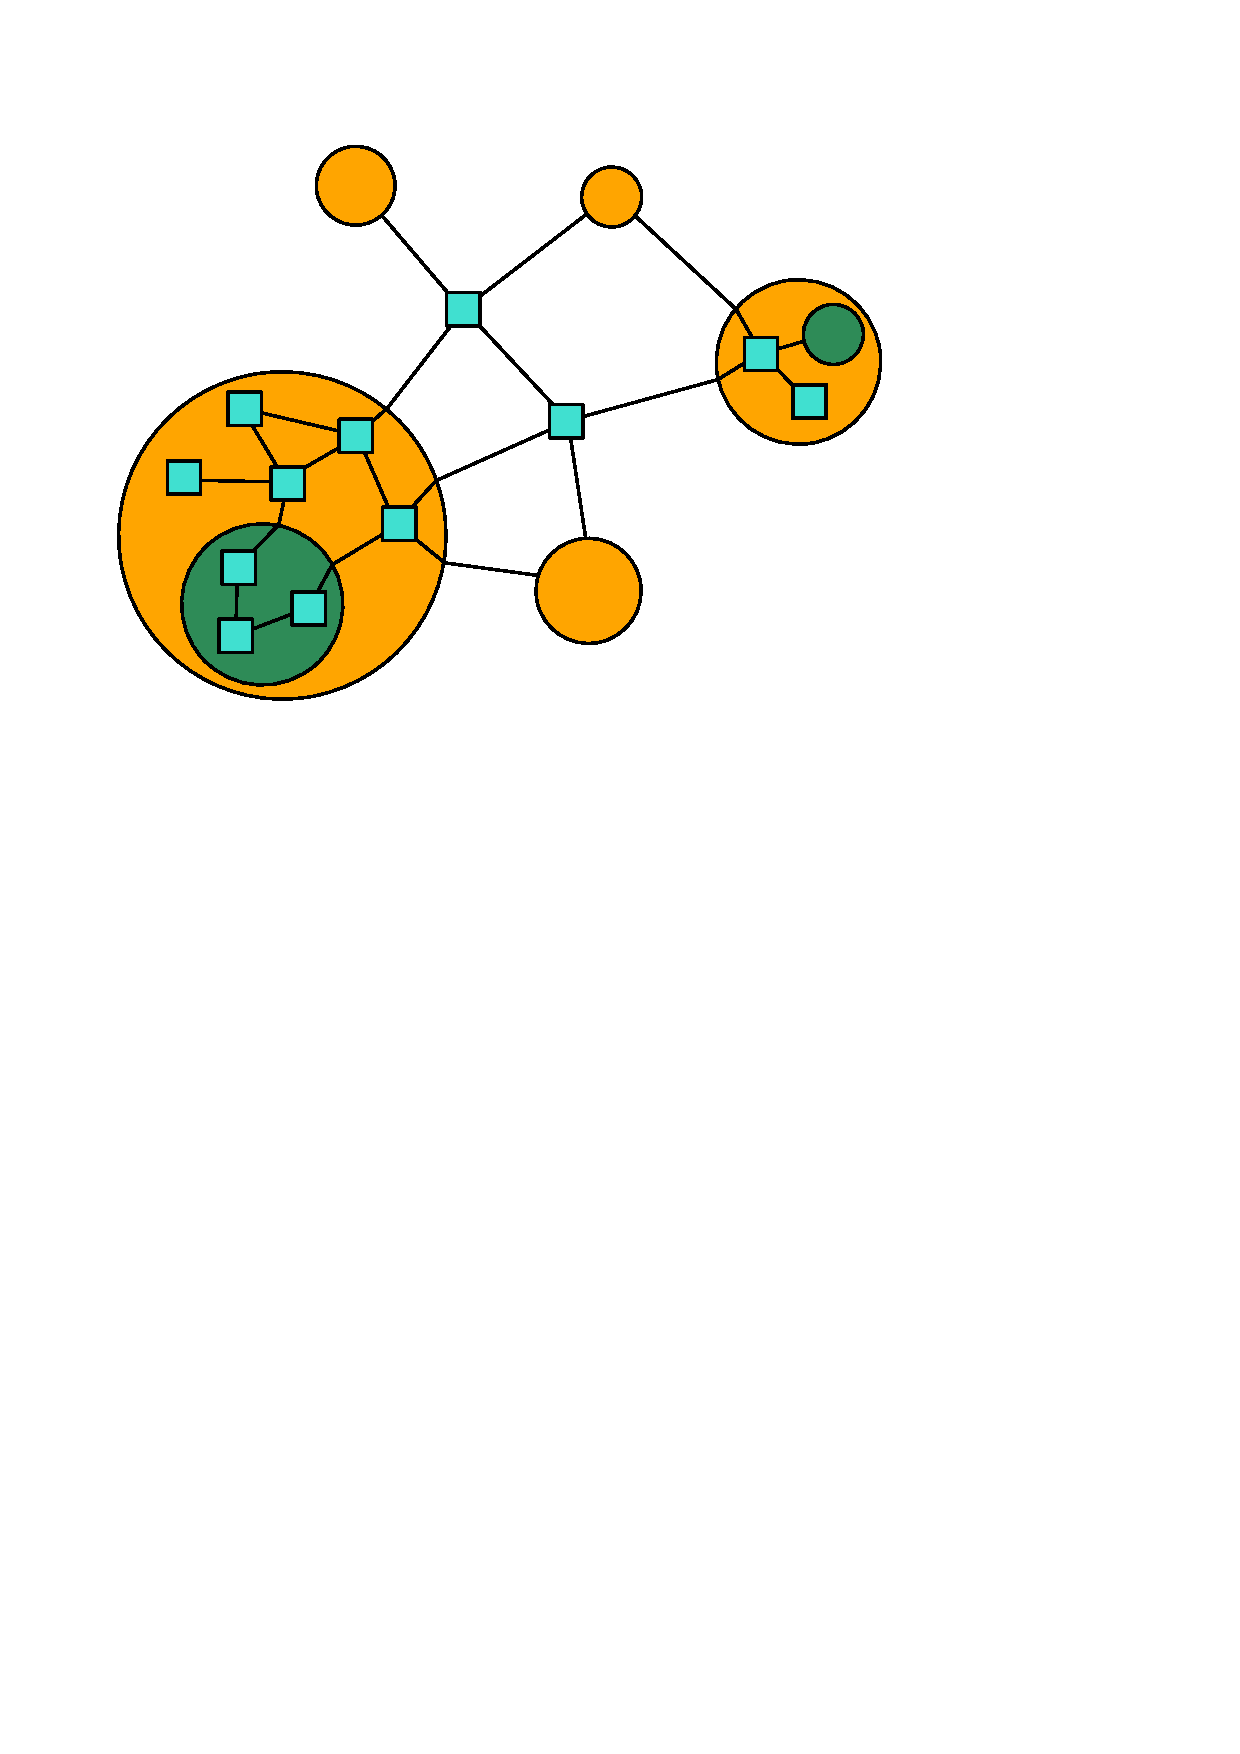
\includegraphics[width=0.7\linewidth]{Pics/Layoutbeispiel.pdf}
  \caption{Beispiellayout einer abstrahierten Argumentkarte nach unserem Konzept.}
  \label{f:Layoutbeispiel}
\end{center}
\end{figure}

% welche Schritte?
Im Folgenden beschreiben wir  in \autoref{sec:Algo} einen Algorithmus um so ein Layout zu berechnen, 
sowie in \autoref{sec:Interaktion} das Konzept um Layoutänderungen bei Interaktionen mit Gruppen gering zu halten.
Zunächst widmen wir uns jedoch kräftebasierten Algorithmen, die wir für unsere Ansätze benutzen, sowie der Größe von geschlossenen Gruppen im Layout.

\myparagraph{Kräftebasierter Algorithmus}
Grundlage für unseren Algorithmus ist die Verwendung eines kräftebasierten Algorithmus. Als Kräfte haben wir unter anderemr die Anziehung adjazenter Knoten bzw. Gruppen,
die Abstoßung zwischen nicht-adjazenten Knoten bzw. Gruppen, sowie die Abstoßung von Knoten selbst, sodass keine adjazenten Elemente die nicht punktförmigen Knoten oder Gruppen schneiden. Außerdem wird eine Abstoßung zwischen Kanten und nicht-inzidenten Knoten bzw. Gruppen benötigt, um Knoten-Kanten-Überschneidungen zu verhindern.
Zusätzlich benötigen wir sogenannte Anker, welche einzelnen Knoten oder Gruppen zugeordnet werden. 
Ein Anker ist ein Pseudoknoten, welcher  nich gerendert wird, sowie eine Kante zu seinem Knoten. 
Anders als normale Kanten ist die optimale Kantenlänge eines Ankers  0. Außerdem ist die Position des Ankers im Layout fest. 
In einem kräftebasierten Algorithmus wirkt der Anker auf seinen Knoten nun wie eine weitere Feder, die ihn zum Ankerpunkt hinzieht.
Die Kraft der Feder kann wie eine normale Kante gehandhabt werden oder bei Bedarf auch anders spezifiziert werden.
Als Grundlage für diesen kräftebasieren Algorithmus könnten man zum Beispiel der Algorithmus von Fruchterman und Reingold \cite{SPE:SPE4380211102} verwenden werden.
Mit nicht punktförmigen Knoten hat sich zum Beispiel bereits Harel und Koren \cite{Harel:2002:DGN:1556262.1556288} beschäftigt.


% Größe geschlossener Gruppen
\myparagraph{Gruppengrößen}
Wie die Größe einer geöffneten Gruppe berechnet werden kann ist in einem späteren Abschnitt genauer beschrieben. 
Eine jedoch vom beschriebenen Algorithmus unabhängige Designentscheidung ist die Größe von geschlossenen Gruppen.
Während eine Möglichkeit wäre, jede geschlossen Gruppe mit einem gleich großen Kreis darzustellen, schlagen wir einen anderen Ansatz vor.

Um direkt zu sehen, ob sich hinter einer geschlossenen Gruppe eine große oder kleine Gruppe bzw. eine mit vielen oder wenigen Kindelemente befindet, empfiehlt es sich den Kreisradius der geschlossenen Gruppe in Beziehung zu der Anzahl der Kindelemente sowie der Größe der Gruppe im offenen Zustand zu setzen.
Da die Größe einer offenen Gruppe stark mit den Anzahl der Kindelemente korreliert, wird dadurch auch diese Eigenschaft einer Gruppe durch die geschlossene Repräsentation
wiedergegeben.
Die Größe der geschlossenen Gruppe könnte also dadurch berechnet werden, dass sie auf einer Skala von einer minimalen bis zu einer maximalen Größe abgebildet wird.
Die minimale Größe könnte hierbei zum Beispiel durch die Größe des am größten dargstellten Arguments gegeben sein und die maximale Größe durch $\gamma \,\%$ 
der größten Gruppe im geöffneten Zustand.

Da der Unterschied zwischen kleinen Gruppen, wobei zum Beispiel eine 4 Kindelemente Besitzt und einer etwas größere die 5 besitzt, stärker verdeutlicht werden soll, als der zwischen 
relativ großen Gruppen, schlagen wir eine logarithmische Abbildung wie in \autoref{f:Radius} vor.
\begin{figure}[h!]
\begin{center} 
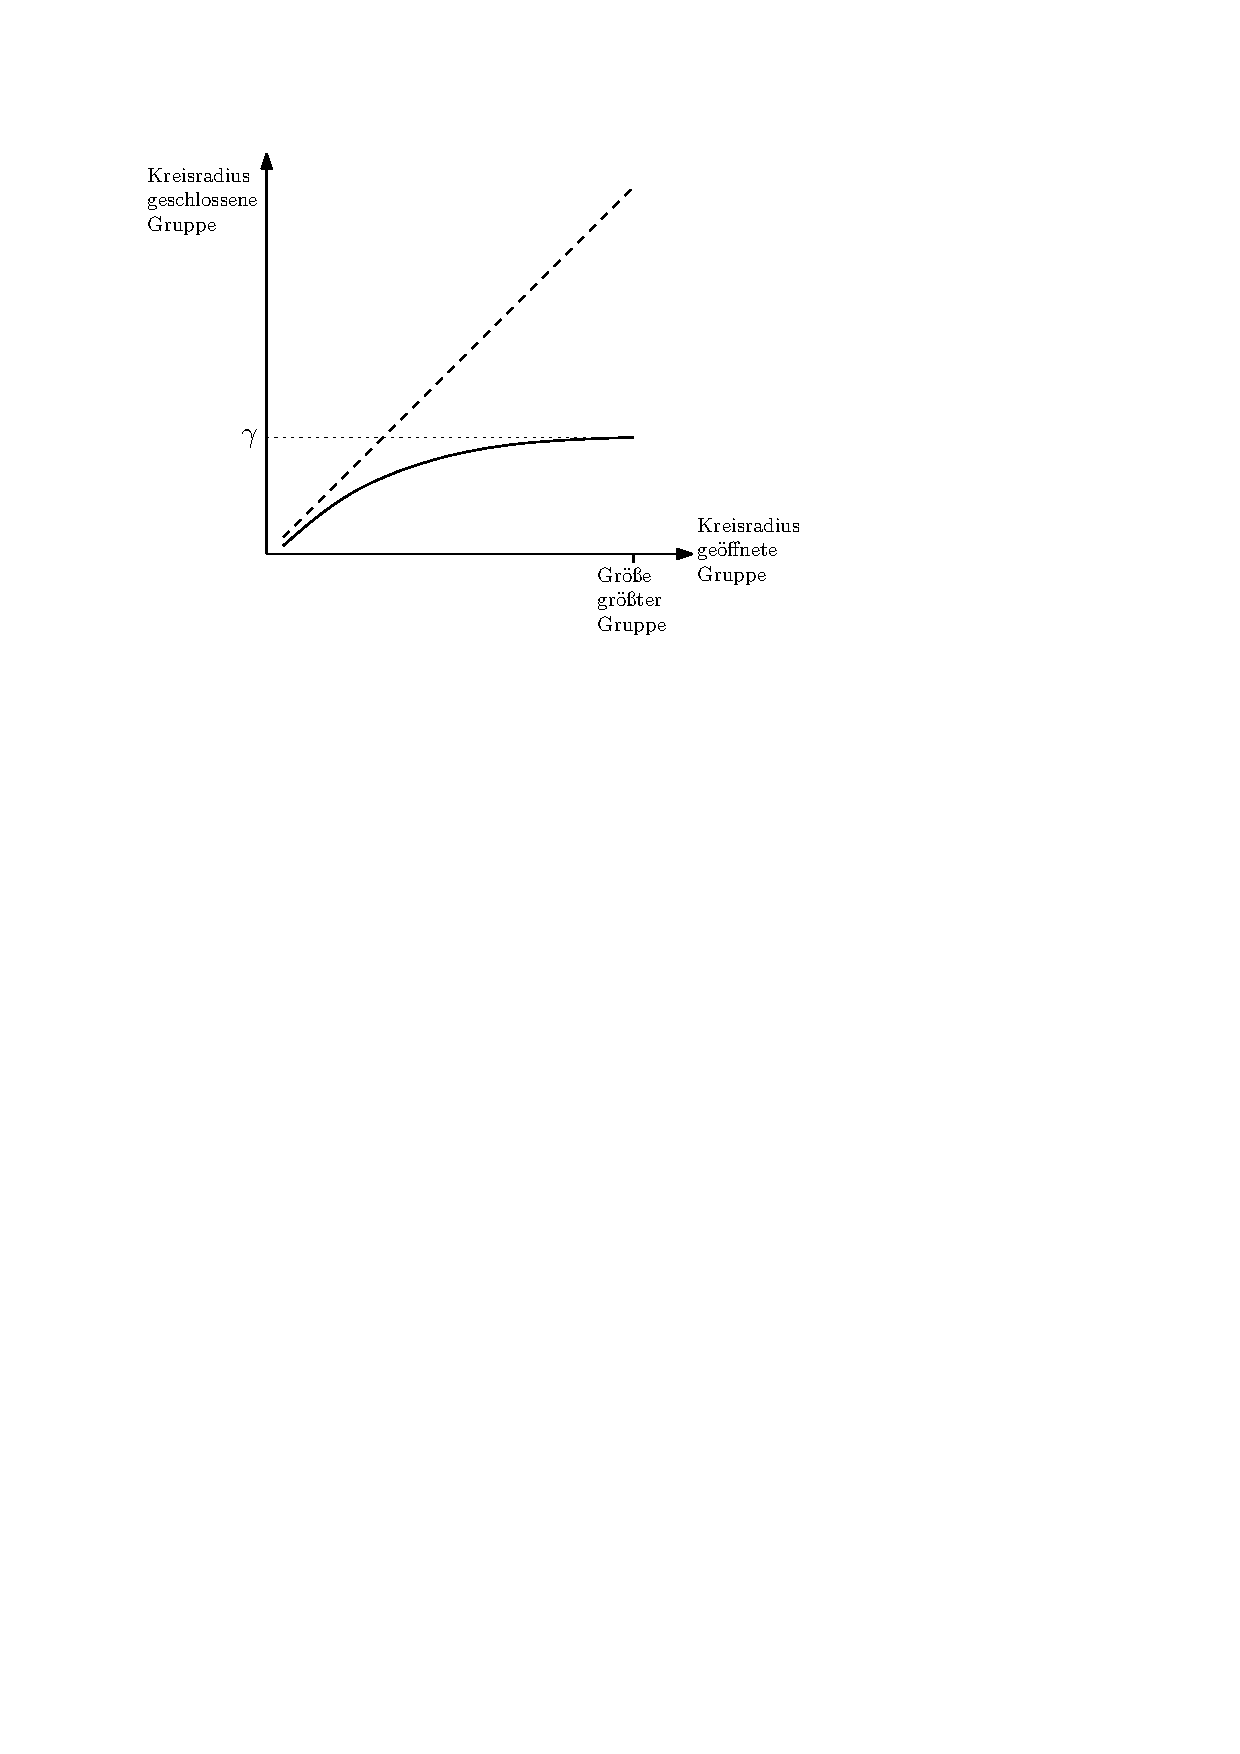
\includegraphics{Pics/Radius.pdf}
% 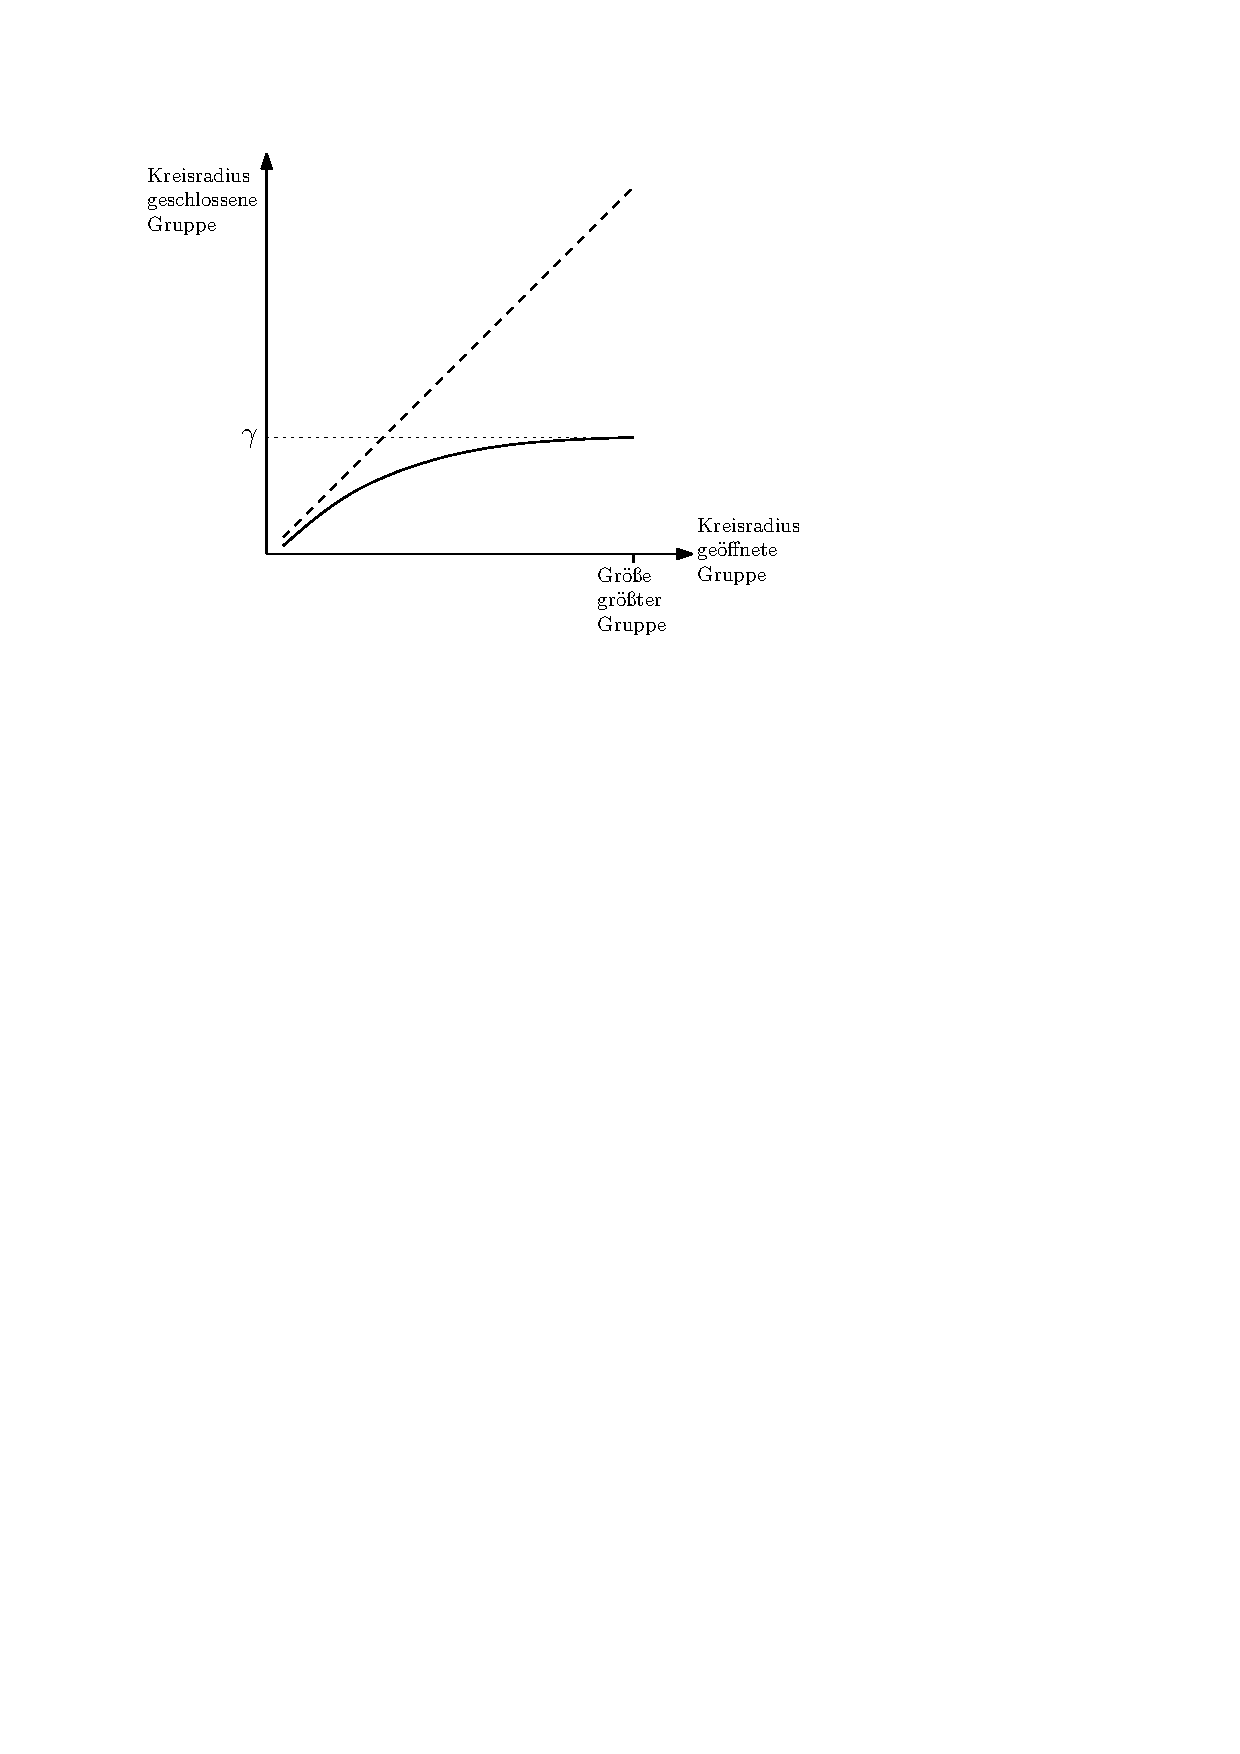
\includegraphics[width=0.5\textwidth]{Pics/Radius.pdf}
  \caption{Vorgeschlagene Wahl der Gruppengröße einer geschlossenen Gruppe in Abhängigkeit der Gruppe in geöffnetem Zustand. }
  \label{f:Radius}
\end{center}
\end{figure}
%\todo[inline]{Gamma Wert weglassen}


\section{Konzept und Idee}
\label{sec:Algo}
% Weitere Constraints für Layout
% Resultat: alle Gruppen geschlossen, jedoch Layout pro Gruppe mit geschlossenen/geöffneten Kind-Gruppen bekannt
Wenn alle Gruppen beim Öffnen einer Karte geschlossen sind, sollte es auf großen Karten einfach sein direkt einen Überblick gewinnen zu können.
Deshalb liefert der folgendes Algorithmus ein Layout bei dem initial alle Gruppen geschlossen sind.

Unser in \autoref{Layoutalgorithmus} grob beschriebene Layoutalgorithmus ist in 2 Phasen unterteilt. 
In der ersten Phase, Zeilen 1-9, werden die in einem bottem-up Ansatz die Größen der Gruppen und erste Layout $\L'$ berechnet. 
Dies beginnt auf der tiefsten Stufe und geht dann iterativ nach oben, da die Größe einer Gruppe jeweils für die Größe der übergordneten Gruppe bzw. obersten Stufe notwendig ist.
In einem top-down Ansatz werden in der zweiten Phase, Zeilen 10-18, nun die Layouts pro Stufe und Gruppe $\L_H$ berechnet und die Ports festgelegt. Das gesamte Layout setzt 
sich dann aus dem Layout der obersten Stufe und den Layouts pro Gruppe zusammen.

\begin{algorithm}[H]
\label{Layoutalgorithmus}
\SetAlgoLined
\Ein{Graph $G=(V,E)$,  Gruppenbaum $T$ } % mit Koten $V$ mit Größe, gerichteten \& gefärbten Kanten $E$, Mengen $S$ von Knoten und Elementen aus $S$
\Aus{Gruppen-hierarchisches Layout von $G$ } % mit diesen und jenen Eigenschaften, evtl Name einführen für Referenzierung
$i =$ niedrigste Stufe einer Gruppe\;
\Solange{$i <$ höchste Stufe}{ 
  \Fuer{Jede Gruppe $H$ auf Stufe $i$} {
	berechnete Layout $\L'_H$ der Gruppe $H$\;
	berechne benötigte Fläche des Gruppenlayouts\;	
  }
  $i= i + 1$\;
}
Berechne Layout auf höchster Stufe\;
Lege Ports für Gruppen auf der zweithöchsten Stufe fest\;
$i =$ zweithöchste Stufe\; 
\Solange{$i \geq$ niedrigste Stufe}{ %Anzahl Stufen % benötigt, dass oberste Ebene auch Gruppe
  \Fuer{Jede Gruppe $H$ auf Stufe $i$} {
	berechnete Layout $\L_H$ der Gruppe $H$ unter Berücksichtigung der Ports\;
	Lege Ports für Gruppen in $H$ auf Stufe $i + 1$ fest;
  }
  $i= i - 1$\;
}
\caption{Layoutalgorithmus}
\end{algorithm}
%\todo[inline]{Algo ist korrigiert muss aber korrekturgelesen werden <- erst Formales klären, Stufen definieren, dann anpassen!}

Im Folgenden beschreiben wir den bottom-up und den top-down Anteil des Algorithmus genauer. 

\subsection{Bottom-up Anteil des Algorithmus}
Schauen wir uns den bottom-up Anteil des Algorithmus genauer an. Ziel ist es zunächst für jede Gruppe ein benötigte Größe zu approximieren.
Da für die Gruppen die Positionen der Ports jedoch noch nicht bekannt sind, werden die Gruppen zunächst ohne Ports gelayoutet.
Hierfür verwenden wir den oben beschrieben kräftebasierten Algorithmus. 
Zusätzlich wird  für jeden Knoten noch ein Anker zu einer relativen Mitte der Gruppe gesetzt. 
Auf Grund der Verwendung eines kräftebasierten Algorithmus hält dies die Gruppe, die nicht zwingend eine Zusammenhangskomponente sein muss, zusammen 
und konzentriert sie in einem eher kreisförmigen Bereich. Anderenfalls könnte sich zum Beispiel eine lange Kette bilden.

Da die Größe von Kindgruppen einer Elterngruppe für deren Layout benötigt wird, beginnt der Algorithmus auf der tiefsten Stufe,
also bei den Gruppen, die in den meisten Gruppen enthalten sind. Wurde ein Layout berechnet, kann ein Kreis darum gelegt werden und somit die Größe approximiert werden.
Mit der oben genannten Rechnung für die Größe von geschlossenen Gruppen, kann nun also die Größe für das Layout eine Stufe höher verwendet werden.
Dies wiederholt sich bis zur obersten Stufe. Hier sind jedoch keine Anker zu einem Mittelpunkt mehr zwingend nötig.
Dies ist nur der Fall, wenn man die gesamte Karte  in einen keisförmigen Bereich ziehen möchte.

\begin{figure}[h!]
\begin{center} 
  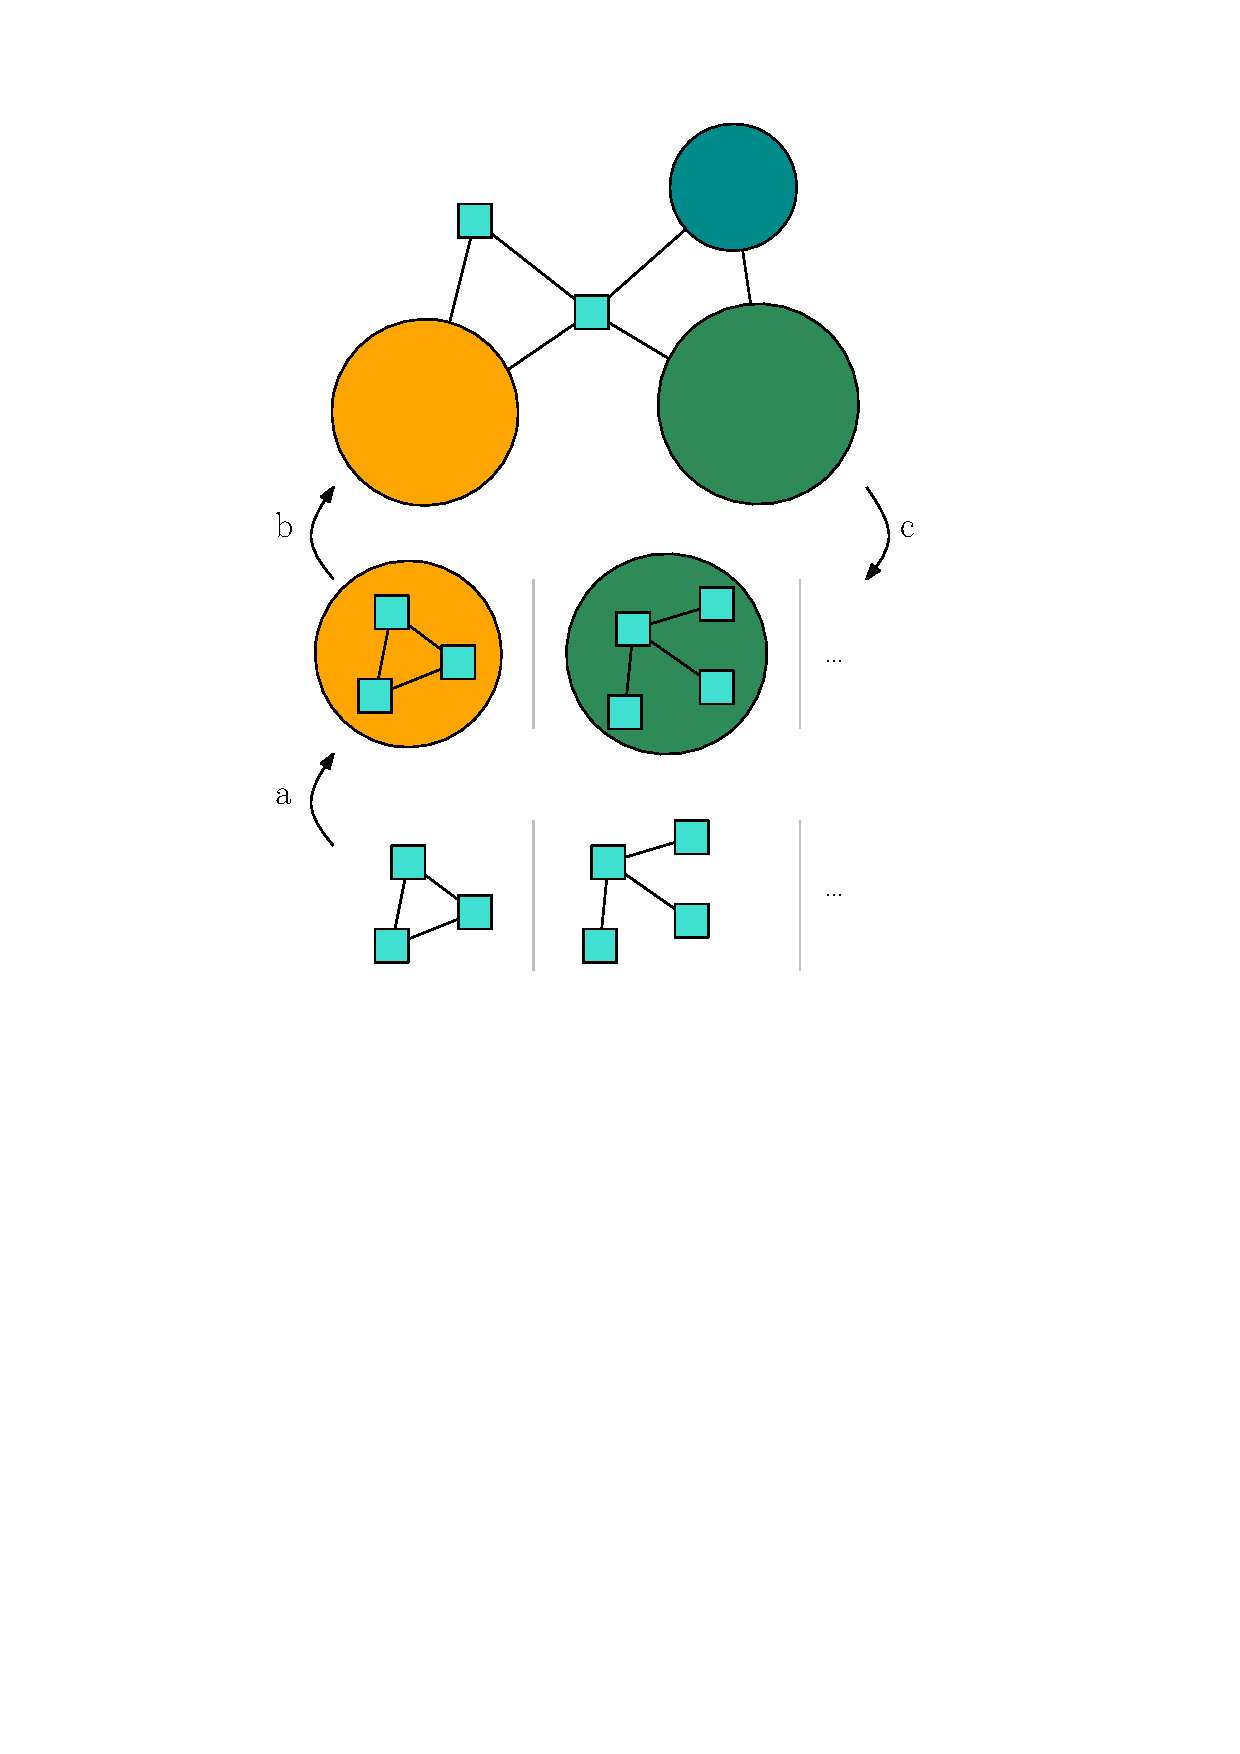
\includegraphics[width=0.5\textwidth]{Pics/BottomUp2.pdf}
  \caption{Bottom-up Anteil des Algorithmus zur Berechnung der benötigten Größen.
  Nachdem Layouts auf der untersten Stufe berechnet wurden (Zeile 4, \autoref{Layoutalgorithmus}) wir in Schritt $a$ die benötigt Größe der Gruppe berechnet (Zeile 5). 
  Nun kann dieser Prozess mit $b$ und $c$ bis zur obersten Stufe wiederholt werden. }
  \label{f:BottomUp}
\end{center}
\end{figure}


\subsection{Top-down Anteil des Algorithmus}
Der Übergang vom bottom-up zum top-down Anteil erfolgt, wenn in Zeile 9 auf der obersten Stufe das Layout berechnet wird.
Wenn zu Beginn, wie bei uns gewählt, alle Gruppen geschlossen sind, dann ist dieses berechnete Layout auch das Layout, das beim Öffnen der Karte zu sehen ist.
Auf der obersten Stufe beginnend und durch das berechnete Layout vorgegeben, legen wir nun die Ports der Gruppen der darunterliegenden Stufe fest und berechnen deren Layouts.

\begin{figure}[h!]
\begin{center} 
  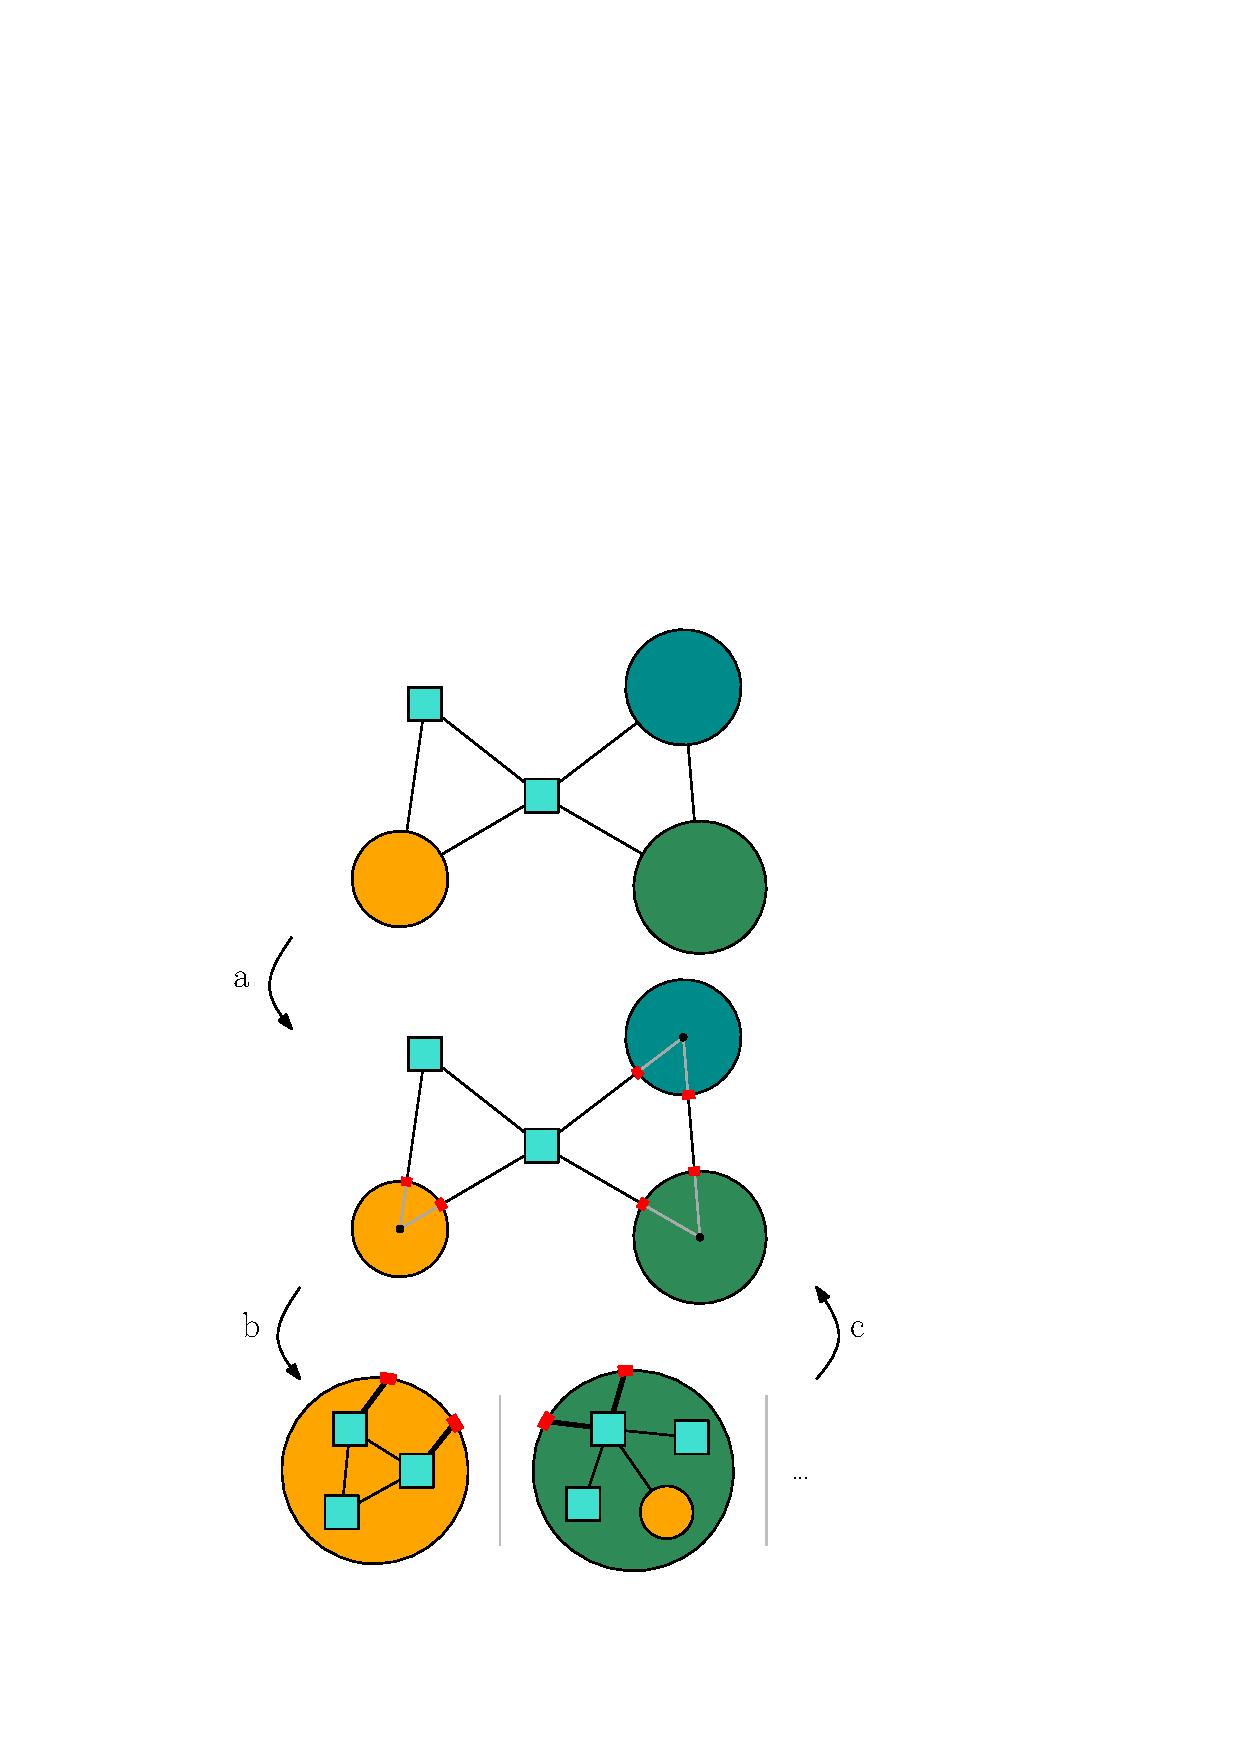
\includegraphics[width=0.5\textwidth]{Pics/TopDown.pdf}
  \caption{Top-down Anteil des Algorithmus zur Festlegung der Ports und Berechnung der Layouts.
  Mit dem Layout der höchsten Stufe können in Schritt $a$ die Ports für die niedrigere Stufe berechnet werden (Zeile 9, \autoref{Layoutalgorithmus}).
  In Schritt $b$ wird dann das Layout der nächsten Stufe mit Ports berechnet (Zeile 13).
  Dieser Prozess mit $b$ und $c$ bis zur untersten Stufe wiederholt werden. }
  \label{f:TopDown}
\end{center}
\end{figure}


%\subsubsection*{Layout in Gruppen in Abhängigkeit von Ports}
% Problem: Layout eines Graphens (mit Labelknoten) innerhalb eines Kreises mit Ports für ausgehende kanten
% Äquivalent: Layout eines Graphens mit punktförmigen Knoten auf Kreis und gelabelten Knoten innerhalb des Kreises
% was betrachten?
Im Folgenden betrachten wir nun die Zeilen 14 und 15 des \hyperref[Layoutalgorithmus]{Layoutalgorithmus~\ref*{Layoutalgorithmus}} genauer. 
% was ist ziel?
Hier ist das Ziel ein Layout für eine Gruppe in Abhängigkeit von bereits gegebenen Ports zu finden, sowie daraufhin dessen Kindgruppen Ports zuzuweisen.
Das heißt, wir suchen nun ein Layout für die Kindknoten einer Gruppe sowie aus der Gruppe herausgehende Kanten.
Dieses soll, wie oben beschrieben, ein Layout innerhalb eines Kreises sein und die Gruppengrenze-überschreitenden Kanten zu den festgelegten Ports führen.
% was ist schwierig?
Eine der Herausforderung hierbei ist, eine geeignete Größe für den Kreis um die Gruppe zu finden. 
Auch zum Finden dieses Layouts benutzen wir wieder den kräftebasierten Algorithmus.

Das bestimmen der Ports ist einfach umzusetzen. 
Wenn ein Layout berechnet wird, werden die Kanten zu einer Gruppe so gelayoutet, dass sie eine inzidente Gruppe nur radial schneiden.
Der erhaltene Schnittpunkt mit dem Kreis der Gruppe legt so die Position für den Port fest, welche einfach durch den Winkel beschrieben werden kann. 
Dies ist auch in Abbildung \autoref{f:TopDown} dargestellt.
Da davon auszugehen ist, dass sich bei Veränderungen im Layout die Winkel nicht zu sehr ändern werden, bleiben die Winkel für jede Gruppengröße fest.
Dadurch bleibt das Layout in einer Gruppe unabhängig von den Änderungen außerhalb. 
Jedoch müssen die verschiedenen Ansätze für das Kantenrouting im verwendeten Algorithmus für die Interaktion beachtet werden.

Für die Layoutberechnung ist eine Gruppe $H$, sowie die vom Layouts der darüberliegenden Stufe bereits festgelegten Ports der Gruppe gegeben.
Diese Ports modellieren wir als feste Knoten auf dem Kreis der Gruppe an ihren jeweiligen Winkeln.
Des Weiteren haben wir bereits ein Layout $\mathcal{L_H}$ der Gruppe $H$ ohne Gruppengrenze-überschreitenden Kanten in Zeile 4 des \hyperref[Layoutalgorithmus]{Layoutalgorithmus~\ref*{Layoutalgorithmus}}  berechnet. 
Aus Zeile 5 haben wir daher auch eine erste Größe für den Kreis der Gruppe, welche durch den Radius beschreiben und durch $R'_H$ gegeben sei. 

Der grobe Ablauf des Algorithmus setzt sich aus drei Schritten zusammen. Zunächst wird ein Anfangslayouts gewählt.
Dann wird ein optimaler Radius  berechnet sowie das Layout berechnet. 
Die Wahl eines Anfangslayouts und das Finden eines optimalen Radius beschrieben wir in den folgenden Abschnitten genauer. 

%\begin{algorithm}[H]
%\label{Gruppenlayoutalgorithmus}
%\SetAlgoLined
%\Ein{Gruppe $H$, sowie Ports und Kanten zu Ports} 
%\Aus{Gruppenlayout $\L_H$ von $H$ }
%Wähle Anfangslayout\;
%Finde Radius $R$ für Kreis\;
%Berechne Gruppenlayout  $\L_H$ mit kräftebasiertem Algorithmus\;
%\caption{Gruppenlayoutalgorithmus}
%\end{algorithm}

Für die Berechnung eines Gruppenlayouts verwenden wir wieder den oben geforderten kräftebasierten Algorithmus, welcher mit Knoten von bestimmter Größer umgehen kann. 
Jedoch schlagen wir auch hier wieder das Hinzunehmen eines Ankers vor, welcher alle Elemente zur Mitte des Kreises ziehen soll.
Dies soll auch verhindern, dass eventuell nicht zusammenhängende Komponenten der Gruppe auseinander driften. 
Die Kraft dieses Ankers sei mit dem Faktor $\alpha$ beschrieben. 
Solange der Kreis der Gruppe groß genug ist, sollte es für Knoten auch nicht möglich sein, aus dem Kreis herausgetragen zu werden. 
Andernfalls müssten man hierfür weitere Kräfte im Algorithmus berücksichtigen oder $\alpha$ entsprechend erhöhen.

% - Anfangslayout: 
\myparagraph{Anfangslayout}
Für die Wahl eines Anfangslayouts schlagen wir folgenden Ansatz vor.
	% c) Layout von Größenberechnung spiegeln (nicht, vertikal, horizontal, beides) und Längen der Port-Knoten-Kanten summieren
In Zeile 4 von \autoref{Layoutalgorithmus} wurde für $H$ bereits ein Layout $\L'_H$ berechnet. 
Dieses lässt sich sowohl horizontal als auch vertikal spiegeln, ohne die Ausrichtung der einzelnen Knoten, welche nach den Achsen ausgerichtete Rechtecke sind, verändert wird.
Das heißt, wir haben vier verschiedene Layouts, nämlich das original, das vertikal oder horizontal gespiegelte sowie das vertikal und horizontal gespiegelte.
Um lange Kanten von Knoten zu Ports durch die ganze Gruppe möglichst zu vermeiden, wählen wir jenes Layout,
bei dem die Summe der Kantenlängen dieser Kanten am kleinsten ist. Dies ist das gewählte Anfangslayout $\mathcal{L}'_H$.
\autoref{f:Anfangslayout} gibt hierfür ein Beispiel.

\begin{figure}[h!]
\begin{center} 
  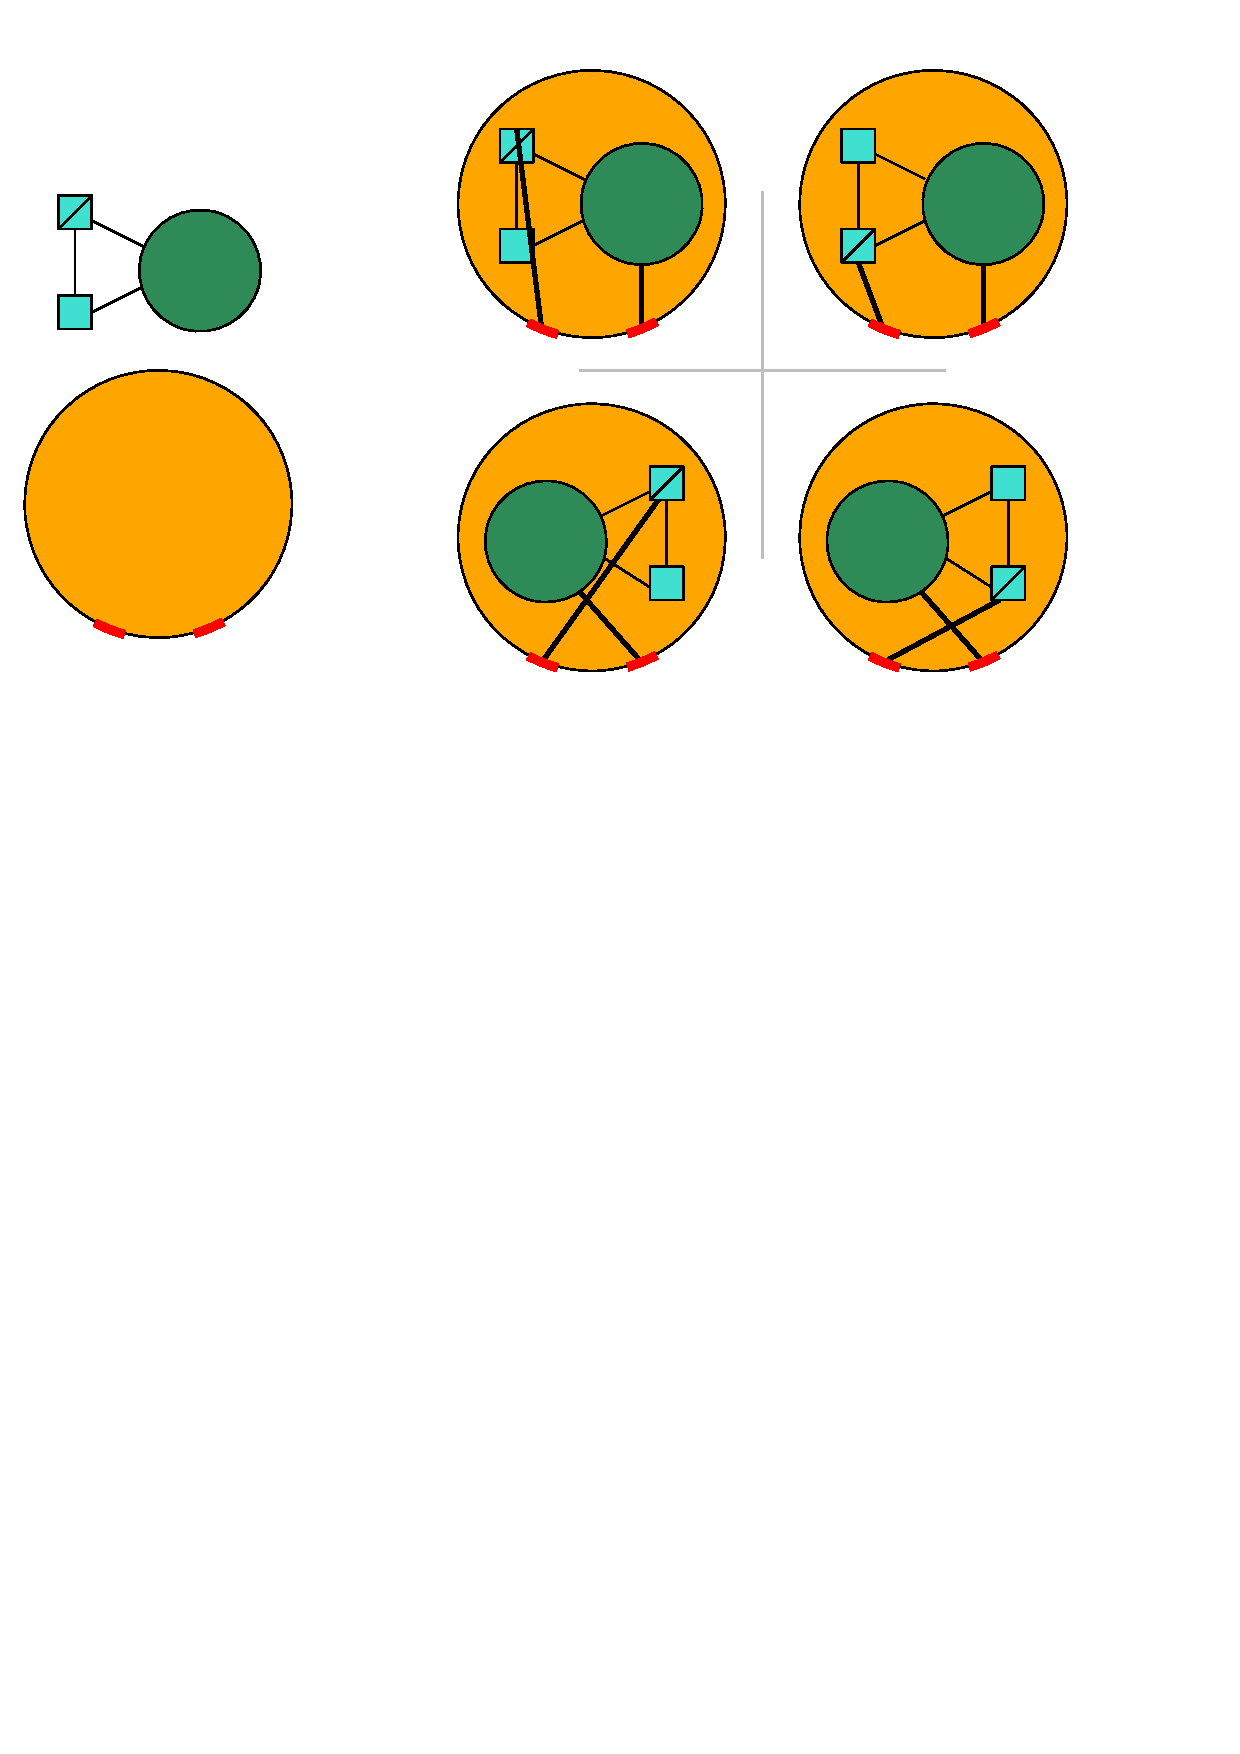
\includegraphics[width=0.8\textwidth]{Pics/Anfangslayout.pdf}
  \caption{Ansatz zur Wahl des Anfangslayouts. Links das vorberechnete innere Layout und die Elterngruppe mit Ports. Rechts die vier verschiedene Spiegelungen des Layouts sowie die Kanten zu den Ports.
  In diesem Fall würde das rechte obere, also horizontal gespiegelte, Layout als Anfangslayout gewählt werden, da die Gesamtlänge der Kanten zu den Ports hier am kürzesten ist.}
  \label{f:Anfangslayout}
\end{center}
\end{figure}

Natürlich gibt es  noch weitere Ansätze zum Finden eines Anfangslayouts.
Einfache Ansätze wären zum Beispiel eine zufällige Platzierung der Knoten oder die Platzierung aller Knoten in die Mitte des Kreises, 
um dann den Rest dem kräftebasierten Layoutalgorithmus zu überlassen. 
Man könnte sich jedoch auch einen anspruchsvolleren Ansatz überlegen, bei dem man das Gruppenlayout ausgehend von den Ports konstruiert.

Mit gewähltem Anfangslayout können wir nun den optimalen Kreisradius einer Gruppe bestimmen.

% - Größe des Kreises definiert durch Radius R
\myparagraph{Bestimmen des Kreisradius einer geöffneten Gruppe}
Für die Berechnung eines angemessenen Kreisradius schlagen wir einen iterativen Algorithmus vor. \label{Radius}
Hierbei führen wir die beiden Schritte Finden des Radius und Berechnen des Layouts zusammen aus.
Die Idee des iterativen Algorithmus ist es, für einen gegeben Radius ein Layout zu berechnen und dann zu testen, ob der Radius verkleinert werden kann.
Ist dies der Fall, so wiederhole das Vorgehen. Ansonsten erhöhe entweder den Faktor $\alpha$ für die Kraft des Ankers zum Mittelpunkt oder breche ab. 
Da hier noch die Anfangsberechnung der Layouts in Gruppen beschreiben wird, ist es wichtig anzumerken, dass die Kindggruppen der behandelten Gruppe 
geschlossen % wieso?
sind.
Wird der Algorithmus später verwendet, muss dies nicht mehr der Fall sein.
\todo[inline]{Wieso geöffnet? Nicht geschlossen sinnvoler? Bei Änderung nachschauen ob oben wo so erwähnt.}

Als Anfangsradius des Algorithmus kann der Radius $R'_H$ aus \autoref{Layoutalgorithmus} Zeile 5 mal einem Faktor $\beta$ verwendet werden.
Die Wahl des Anfangslayouts haben wir im Abschnitt davor beschrieben.

\begin{algorithm}[H]
\label{Kreisradiusalgorithmus}
\SetAlgoLined
\Ein{Gruppe $H$, Ports, Kanten zu Ports, Anfangslayout $\L'_H$, Radius $R'_H$}
\Aus{Gruppenlayout $\L_H$ von $H$, Radius $R_H$}
$R = \beta \cdot R'_H = $ Anfangsradius für Kreis\;
$\L_H = \L'_H \cup$ Ports $\cup$  Kanten zu Ports\;
Führe kräftebasiertem Algorithmus auf  $L_H$ aus\;
\eWenn{$R$ verkleinert werden kann}{
	Passe $R$ an\;
}{
	\eWenn{$\alpha$ nicht zu groß}{
		erhöhe $\alpha$\;
		gehe zu 3\;
	}{
		Algorithmus fertig\;
	}
}
\caption{Kreisradiusalgorithmus}
\end{algorithm}

Für \autoref{Kreisradiusalgorithmus} muss natürlich noch spezifiziert werden, was es heißt, dass der Radius in Zeile 4 verkleinert werden kann
oder dass $\alpha$ nicht zu groß ist. 
Dass der Radius $R$ verkleinert werden kann, soll bedeuten, dass bei kleinerem $R$ aber gleichem Layout der Kreis keine Knoten schneidet. 
Typisch für Parameter bei kräftebasierten Algorithmen, wird um eine geeignete maximale Größe von $\alpha$ zu finden, wohl eine Implementierung und verschiedene Tests benötigt. 
Dasselbe gilt für $\beta$ um einen geeigeneten Anfangsradius zu finden.

Eine weitere Variante zur Berechnung des Kreisradius könnte durch erwartete Größe von Gruppen umgesetzt werden. 
Falls ein gutes $\beta$ gefunden werden kann, dass für jede Gruppe eine gute Größe approximiert und dabei nie zu klein ist, kann der iterative Prozess auch ausgelassen werden
und der Radius der Gruppe für jeden Zustand direkt berechnet werden.			

% Anmerkung: Da in Praxis (Argumentkarten) die Gruppentiefe nicht hoch ist und in Gruppe nicht viele Gruppen sind, 
			% können hier auch die Größen für alle Fälle berechnet werden
% Postprocessing: Kantenklätung

Abschließend zur Beschreibung der Layoutberechnung wollen wir anmerken, dass die bottom-up und top-down Anteile auch wiederholt durchgeführt werden können.
Dadurch können die benötigten Größen in den Layoutberechnungen besser berücksichtigt werden und so auch die resultierende Ports besser festgelegt werden.

%---------------------------------------------------------------------------------------------
\section{Layout-Anpassung bei Interaktion}%statt: m Öffnen oder Schließen einer Gruppe}
% was betrachten?
\label{sec:Interaktion}
Nachdem ein Anfangslayout für die ganze Argumentkarte gefunden wurde, bei der alle Gruppen geschlossen sind, möchte man nun auch Gruppen öffnen. 
Das Layout für jede Gruppe wurde ebenfalls bereits berechnet. Zur Erinnerung, wenn eine Gruppe geschlossen ist, hat sie eine Größe, 
die Abhängig von der Größe im offenen Zustand kleiner ist. 
Da diese Gruppe im geöffneten Zustand nun jedoch mehr Platz einnimmt ergibt sich folgende Problemstellung:
% was ist ziel?
Wie verändert sich das Layout auf darüberligenden Stufen, wenn eine Gruppe geöffnet oder geschlossen wird? 
Hierbei wird wie spezifiert außerdem gefordert, dass die Änderungen im Layout nicht zu stark sind, 
damit man sich mit seiner mentalen Karte von vor der Änderung auch danach noch zurechtfindet.
% was ist schwierig?

Der von uns vorgeschlagene Lösungsansatz basiert erneut auf einem kräftebasierten Algorithmus. 
Auch hier verweisen wir auf den oben beschriebenen Algorithmus. Es gibt zwei Probleme zu lösen. 
Zum Einen, wie groß ist eine Gruppe in ihrem jetzigen Zustand.  
Zum Anderen, wie man dafür sorgt, dass sich das Layout nach Öffnen oder Schließen einer Gruppe nicht zu sehr verändert.

% Ansatz für Größe
Um die Größe einer Gruppe in ihrem jetzigen Zustand zu berechnen, könnte man verschieden vorgehen. 
Zum Beispiel könnte man ihn aus den bekannten Radien, für den Zustand alle Untergruppen geöffnet und der Gruppe selbst geschlossen, berechnen. 
Oder aber man benutzt den Algorithmus aus dem vorherigen Abschnitt, um ihn entweder im Vorraus oder wenn benötigt zu ermitteln. 
Wird nun eine Gruppe geöffnet oder geschlossen, wird diese durch eine größere bzw. kleinere ersetzt. 
Diese Änderung zieht sich logischer Weise bis zur obersten Stufe durch.

Um das Verhalten bei einer Interkation mit einer Gruppe zu kontrollieren, erweitern wir den verwendeten kräftebasierten Layoutalgorithmus um mehrere Anker. 
Dies geschieht pro Stufe und Gruppe für die ein neues Layout berechnet werden muss.
Jedes gelayoutet Element, was sich also nicht in einer geschlossenen Gruppe befindet, bekommt einen Anker gesetzt und zwar an der Position, 
an der es sich im Anfangslayout der Gruppe bzw. obersten Stufe befindet. 
Diese Anker bezeichnen wir als Grundanker. 
Wenn nun eine Gruppe geöffnet oder geschlossen wird und die dadurch verursachten Größenänderungen pro Stufe durchgeführt wurden, 
wird in jeder veränderten Gruppe sowie der obersten Stufe der Layoutalgorithmus mit den zuvor gesetzten Grundankern gestartet. 
Dies wird  durch \autoref{f:Interaktion} veranschaulicht. 
Die Grundanker sorgen nur dafür, dass die Elemente nicht zu stark von ihrer Position vor der Veränderung verschoben werden.

\begin{figure}[h!]
\begin{center} 
  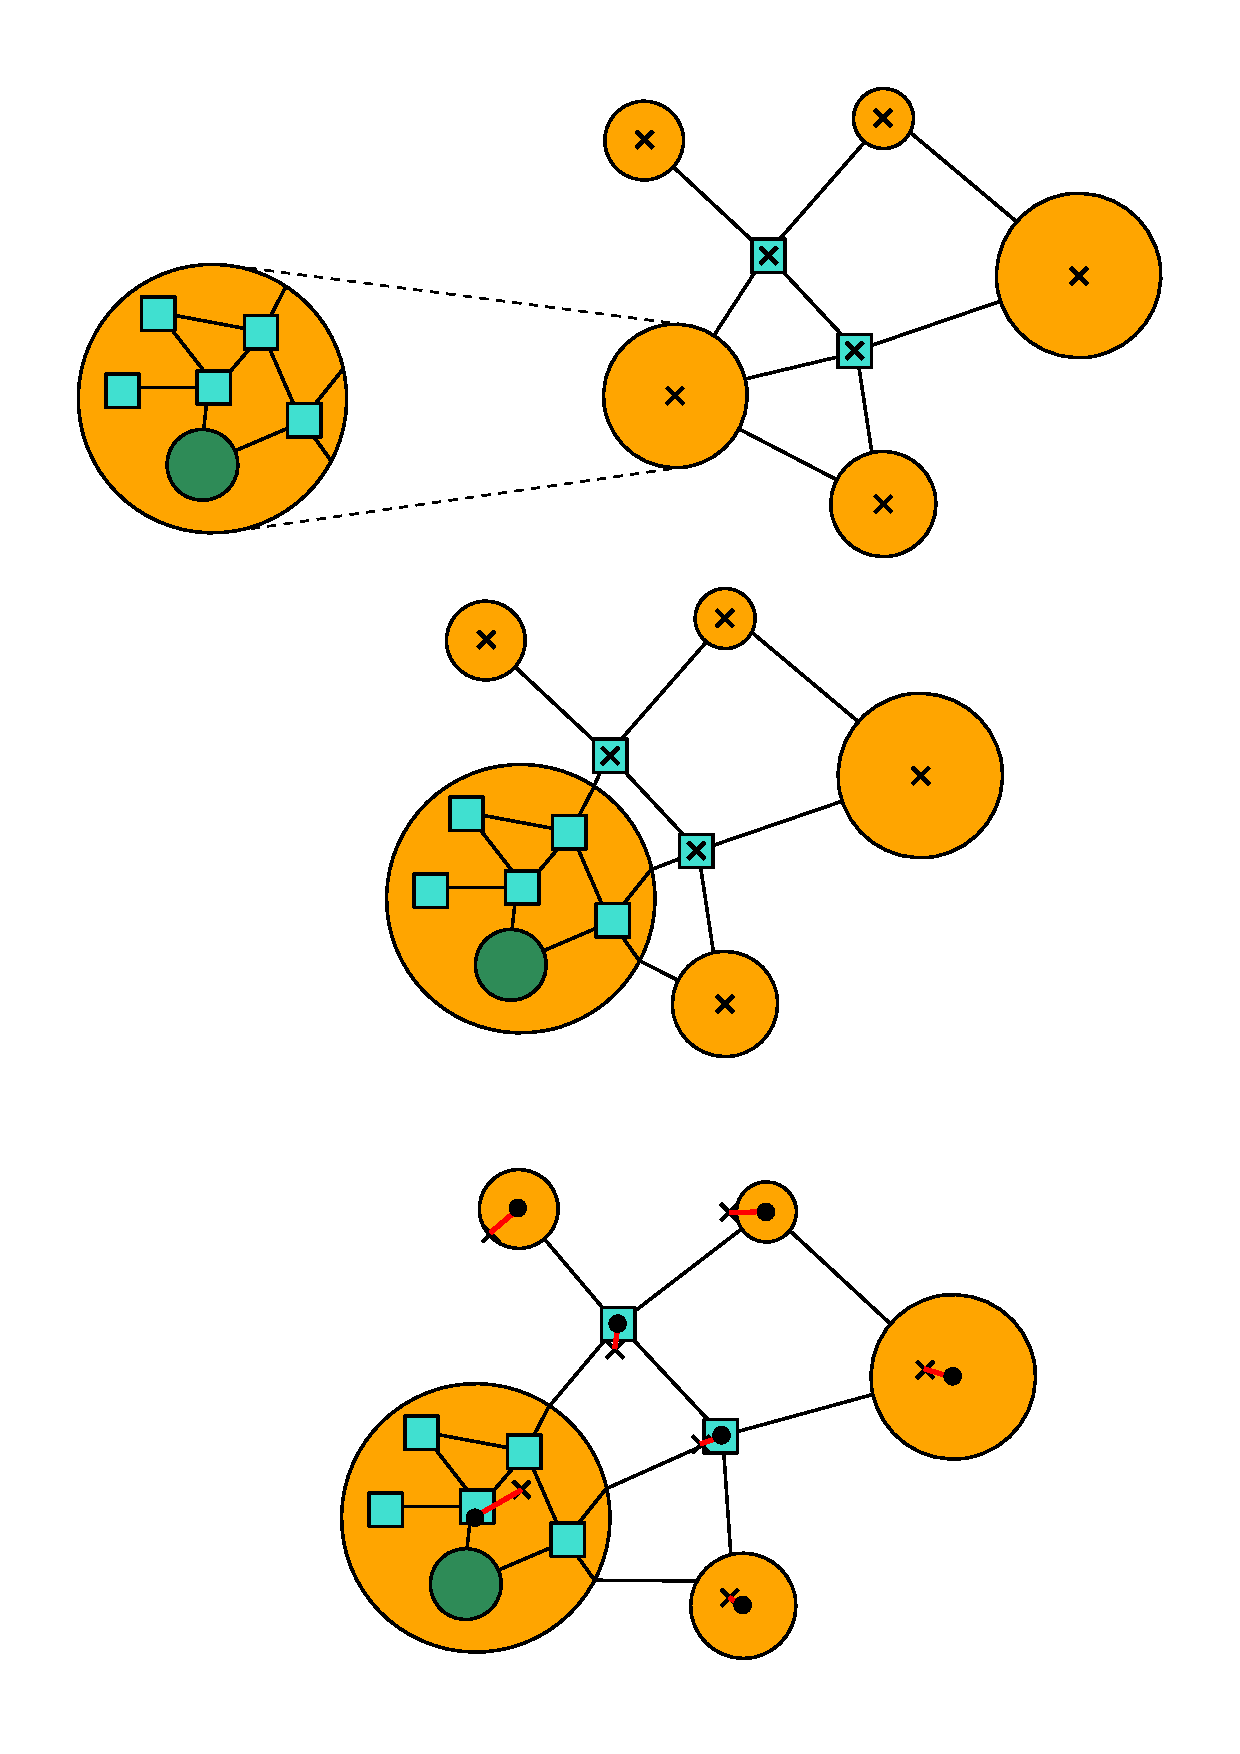
\includegraphics[width=0.7\textwidth]{Pics/Interaktion.pdf}
  \caption{Veranschaulichung des Ankerprinzips beim Öffnen einer Gruppe.}
  \label{f:Interaktion}
\end{center}
\end{figure}

Genauer zu spezifizieren ist, wie stark die Anker sein sollten sowie ob sie von der Gruppen- bzw. Elementgröße abhängig sein sollten. 
Hierfür sind erneut eine Implementierung sowie Tests nötig. Dies Wahl könnte natürlich auch sehr von der Argumentkartenstruktur sowie der eigenen Vorliebe abhängen.

Durch das Öffnen vieler Gruppen können große Veränderungen zum Grundlayout zustande kommen.
Die Kräfte der Anker könnten so im Verhältnis zu anderen Kräften zu stark werden und unschöne Layouts erzeugen.
Deshalb ist ein weiterer Punkt bei diesem Lösungsansatz, dass in einem solchen Fall die Grundanker ignoriert werden 
und lediglich temporär neue Anker vor der letzten Änderung gesetzt werden. 
Es wird also nur versucht zum letzten Layout die Veränderungen gering zu erhalten, nicht jedoch direkt zum Anfangslayouts. 
Wann dieser Fall eintritt muss noch genauer spezifiert werden und kann pro Stufe unterschiedlich gehandhabt werden.

% ------- Vorgehen für Parameterwahl vorschlagen
%\todo[inline]{Vorgehen für Parameterwahl vorschlagen?}


\chapter{Evaluation und Vergleich zu anderen Lösungsansätzen}
\label{chapter:vgl}

Bei der Entwicklung unserer Lösung sind noch andere Ansätze entstanden, welche nach Evaluation mit unserem Ansatz aus \autoref{chapter:algo}, aber nicht weiter ausgearbeitet oder ausgewertet wurden. Für die Vollständigkeit stellen wir nun noch kurz einen alternativen kräftebasierten Ansatz (siehe \autoref{UniformK-Ansatz}) und einen hierarchischen Ansatz (siehe \autoref{Hierarch-Ansatz}) vor. Ein kurzer Vergleich wird in \autoref{Ansatz-Vergleich} gezeigt.

\section{Uniform kräftebasiertes Layout}
\label{UniformK-Ansatz}
Dieser Lösungsansatz stellt eine einfache Erweiterung zu vorhandenen kräftebasierten Algorithmen dar: Knoten können durch zusammenfassende Pseudoknoten in diesem Fall, Gruppenknoten, repräsentiert werden und es werden zusätzlich Anker verwendet.

Konkret bedeutet dies, dass Knoten zunächst nur durch ihre zusammengefassten Pseudoknoten darstellt werden und hierfür mit einem einfachen kräftebasierten Verfahren ein Layout bestimmen, wobei die abstoßende Kraft der Pseudoknoten bzw. die Anziehungskraft zusammengelegter Kanten logarithmisch mit der Anzahl zusammengefassten Elemente skaliert wird.

Wenn nun die Elemente einer oder mehrerer Gruppen konkret dargestellt werden sollen, so werden die Pseudoknoten zunächst ähnlich wie bei der finalen Lösung verankert. Zusätzlich werden die Pseudoknoten deren Elemente dargestellt werden sollen aus dem Layout entfernt und stattdessen die Knoten der Gruppe, die ebenfalls Pseudoknoten für innere Gruppen sein können, eingefügt. Schließlich wird nun noch einmal der kräftebasierte Algorithmus verwendet mit der Besonderheit, dass jeder Knoten eine zusätzliche Anziehung zu seinem Anker bzw. dem Anker des übergeordneten Pseudoknotens.

Dieser Ablauf wird in \autoref{UniformK-Skizze} skizziert.

\begin{figure}[h!]
\begin{center}
	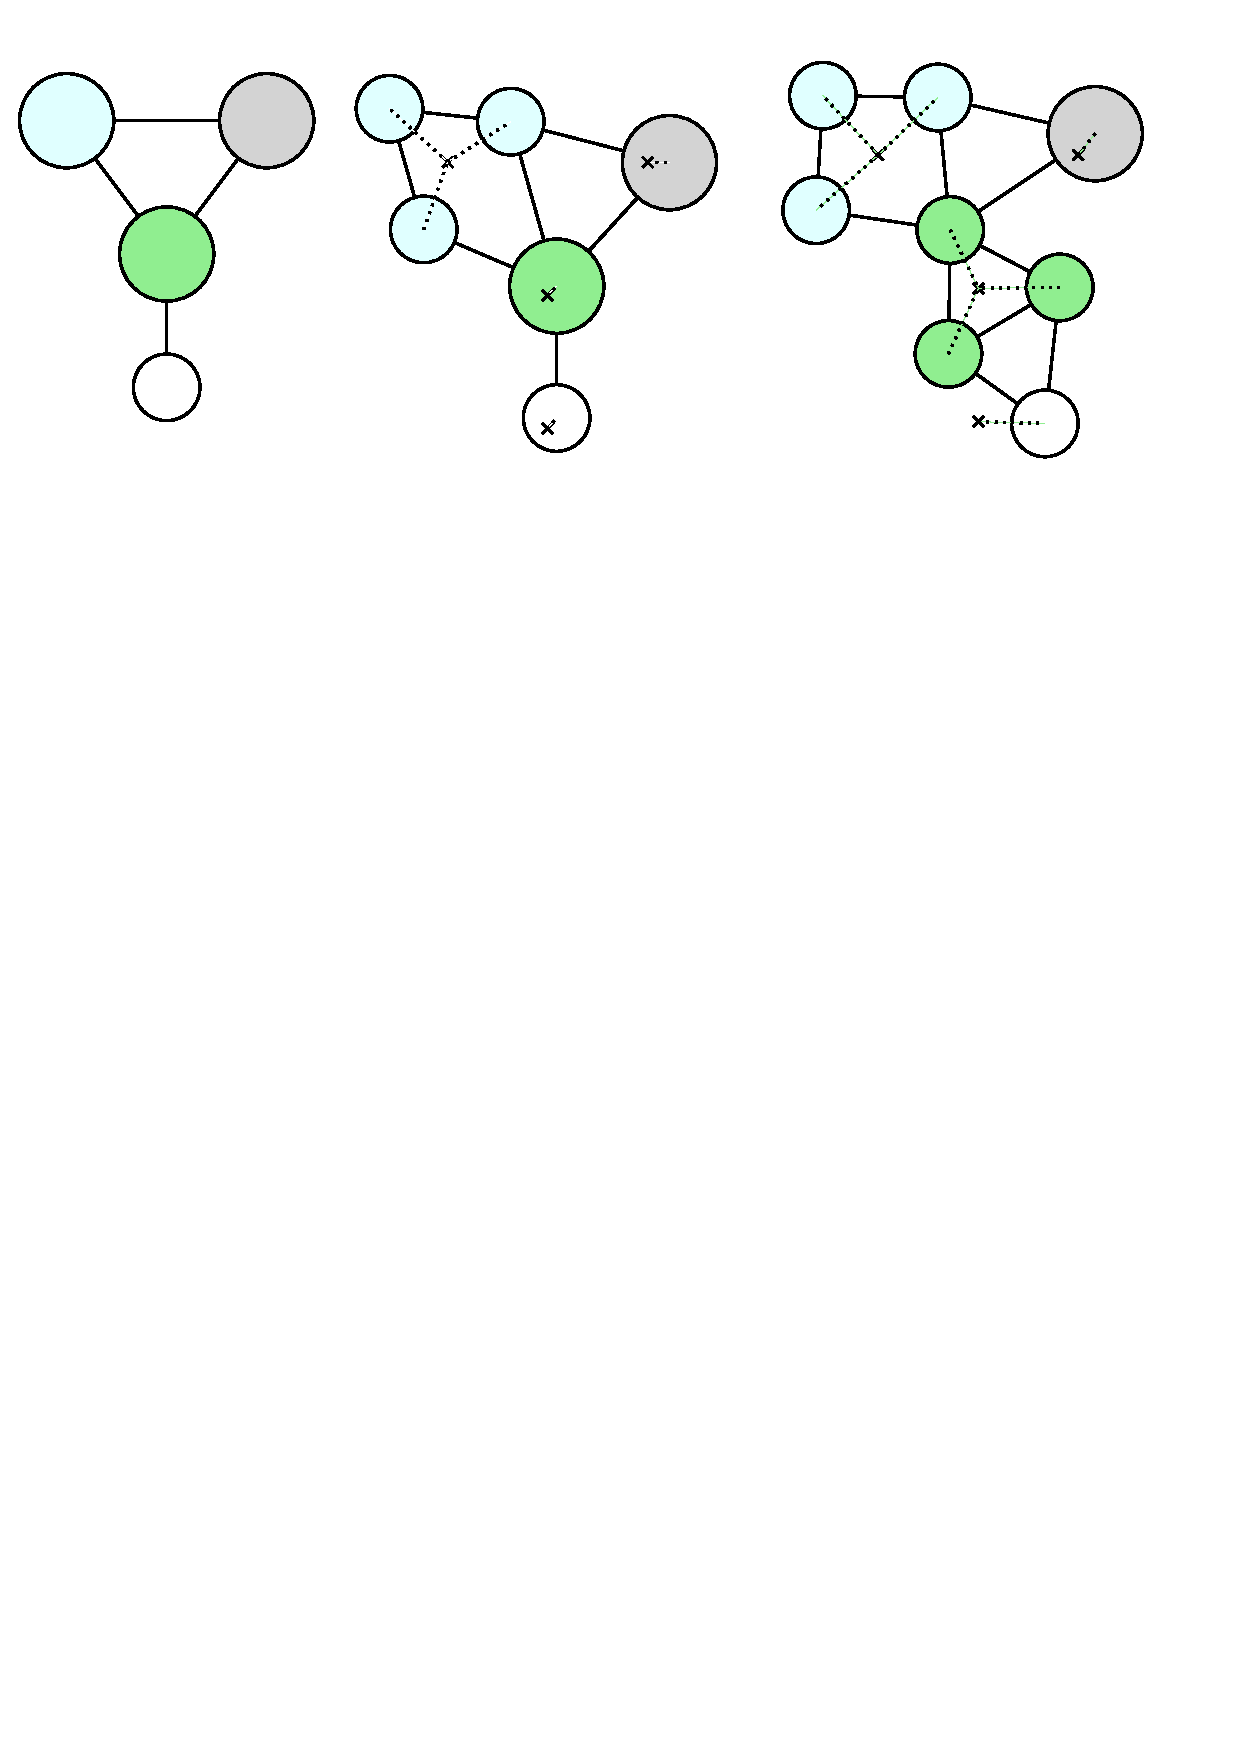
\includegraphics[width=\textwidth]{Pics/uniform_kb.pdf}
	\caption{Skizze eines Layouts durch den uniform krqftebasierten Ansatz. Links zunächst das Layout mit alle Gruppen geschlossen. In der Mitte das Layout nach Öffnen der hellblauen Gruppe. Rechts das Layout mit hellblauer und grüner Gruppe geöffnet. Kreuze markieren hierbei die Anker der Gruppen.}
	\label{UniformK-Skizze}
\end{center}
\end{figure}

% zu vergleichen mit hierarchischem Layout und alles kräftebasiert

\section{Hierarchisches Layout}
\label{Hierarch-Ansatz}
Häufig auftretende Eigenschaften in Argumentkarten wie Zyklenfreiheit legen andere Graphenlayouts, insbesondere hierarchische Layouts, nahe.

Wenn wir die Richtung der Kanten, entgegen der bisherigen Ansätze, für das Layout beachten wollen, wird es dadurch möglich bei einem hierarchischen Layout alle eingehenden Kanten eines Knotens an der Oberseite des Knotens und alle ausgehenden Kanten an der Unterseite des Knotens zu zeichnen. Dadurch wird ebenfalls das \glqq einpacken \grqq\ der Knoten in eine Box zur Repräsentation bzw. Ordnung der Gruppe einfacher, da auch die Box der Gruppe die ein- und ausgehenden Kanten entsprechend ordnen kann ohne die Komplexität des Layouts innerhalb der Box zu erhöhen, wodurch das innere und äußere Layout von Gruppen getrennt berechnen werden können.

Ein grobe Skizze zu einem solchen Layout ist in \autoref{Hierarch-Skizze} dargestellt.

\begin{figure}[h!]
\begin{center}
	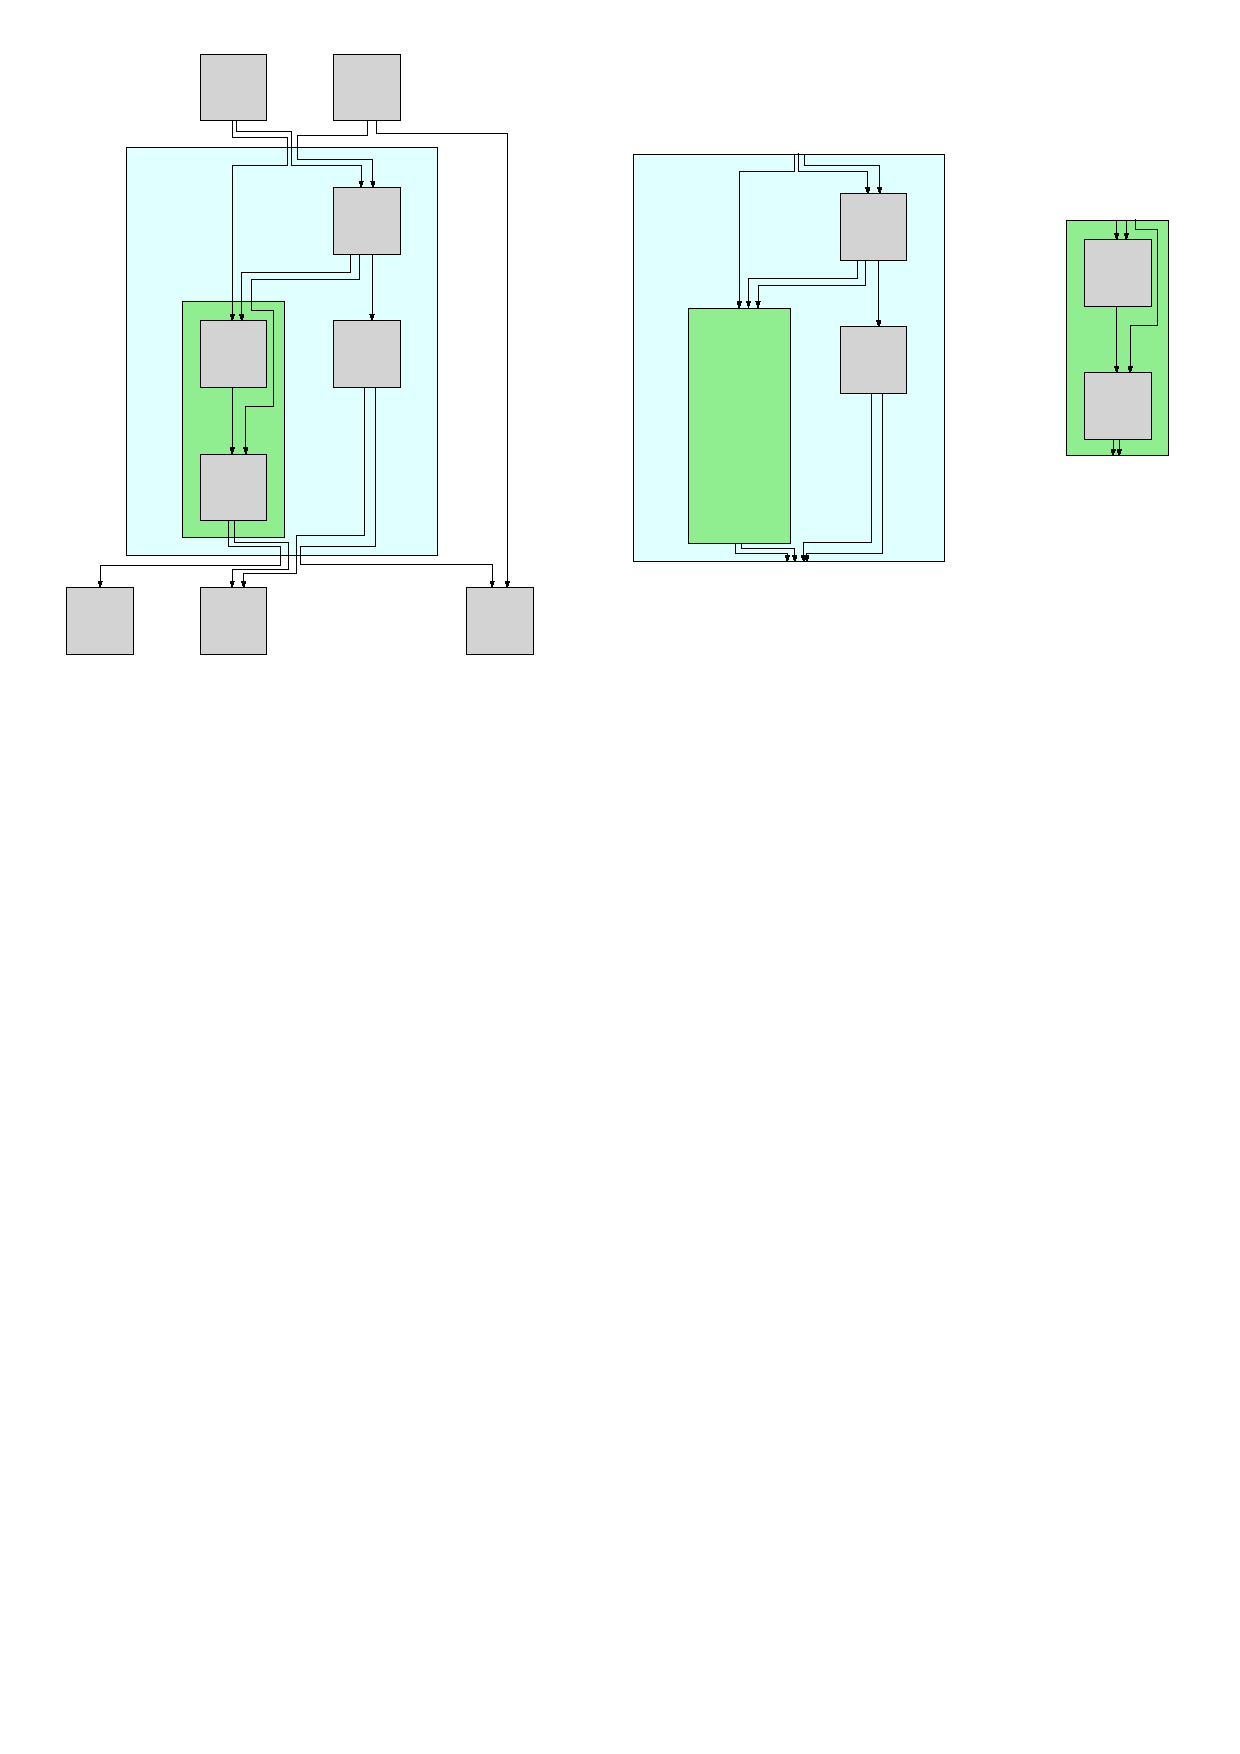
\includegraphics[width=\textwidth]{Pics/hierarchisch.pdf}
	\caption{Skizze eines Layouts durch den hierarchischen Ansatz. Links das Gesamtlayout, Mitte und Rechts jeweils das Layout der jeweiligen Gruppe.}
	\label{Hierarch-Skizze}
\end{center}
\end{figure}

\section{Vergleich}
\label{Ansatz-Vergleich}
Da keiner der Ansätze konkret implementiert wurde und die alternativen Ansätze auch stückweise ausgearbeitet wurden, besteht der Vergleich dieser Ansätze größtenteils aus Abschätzungen und nicht tatsächlichen Messungen. Es werden folgende Abkürzungen verwendet:

\textbf{KBK}: Unser Lösungsansatz, der kräftebasierte Algorithmus mit Kapselung

\textbf{HL}: Der hierarchische Layout-Ansatz

\textbf{UKB}: Der uniform kräftebasierte Layout-Algorithmus

\paragraph*{Fokus des Layouts}
Bei KBK und HL sind die Layouts der einzelnen Gruppenebenen größtenteils unabhängig, daher liegt der Fokus der Darstellung eher auf der Semantik der Gruppen, d.h. das Layout stellt besonders heraus, zu welcher Gruppe ein Knoten gehört.

Das durch UKB erzeugte Layout basiert dagegen größtenteils auf den Knotenzusammenhängen ab. Durch die Anker bleiben Gruppenelemente zwar größtenteils zusammen, aber das Layout wird dennoch über die Kanten der Knoten in und zwischen Gruppen festgelegt. Bei entsprechenden Zusammenhängen können Gruppen auch deformiert oder getrennt werden (siehe \autoref{Uniform-Trenn-Skizze}).

\begin{figure}[h]
\begin{center}
	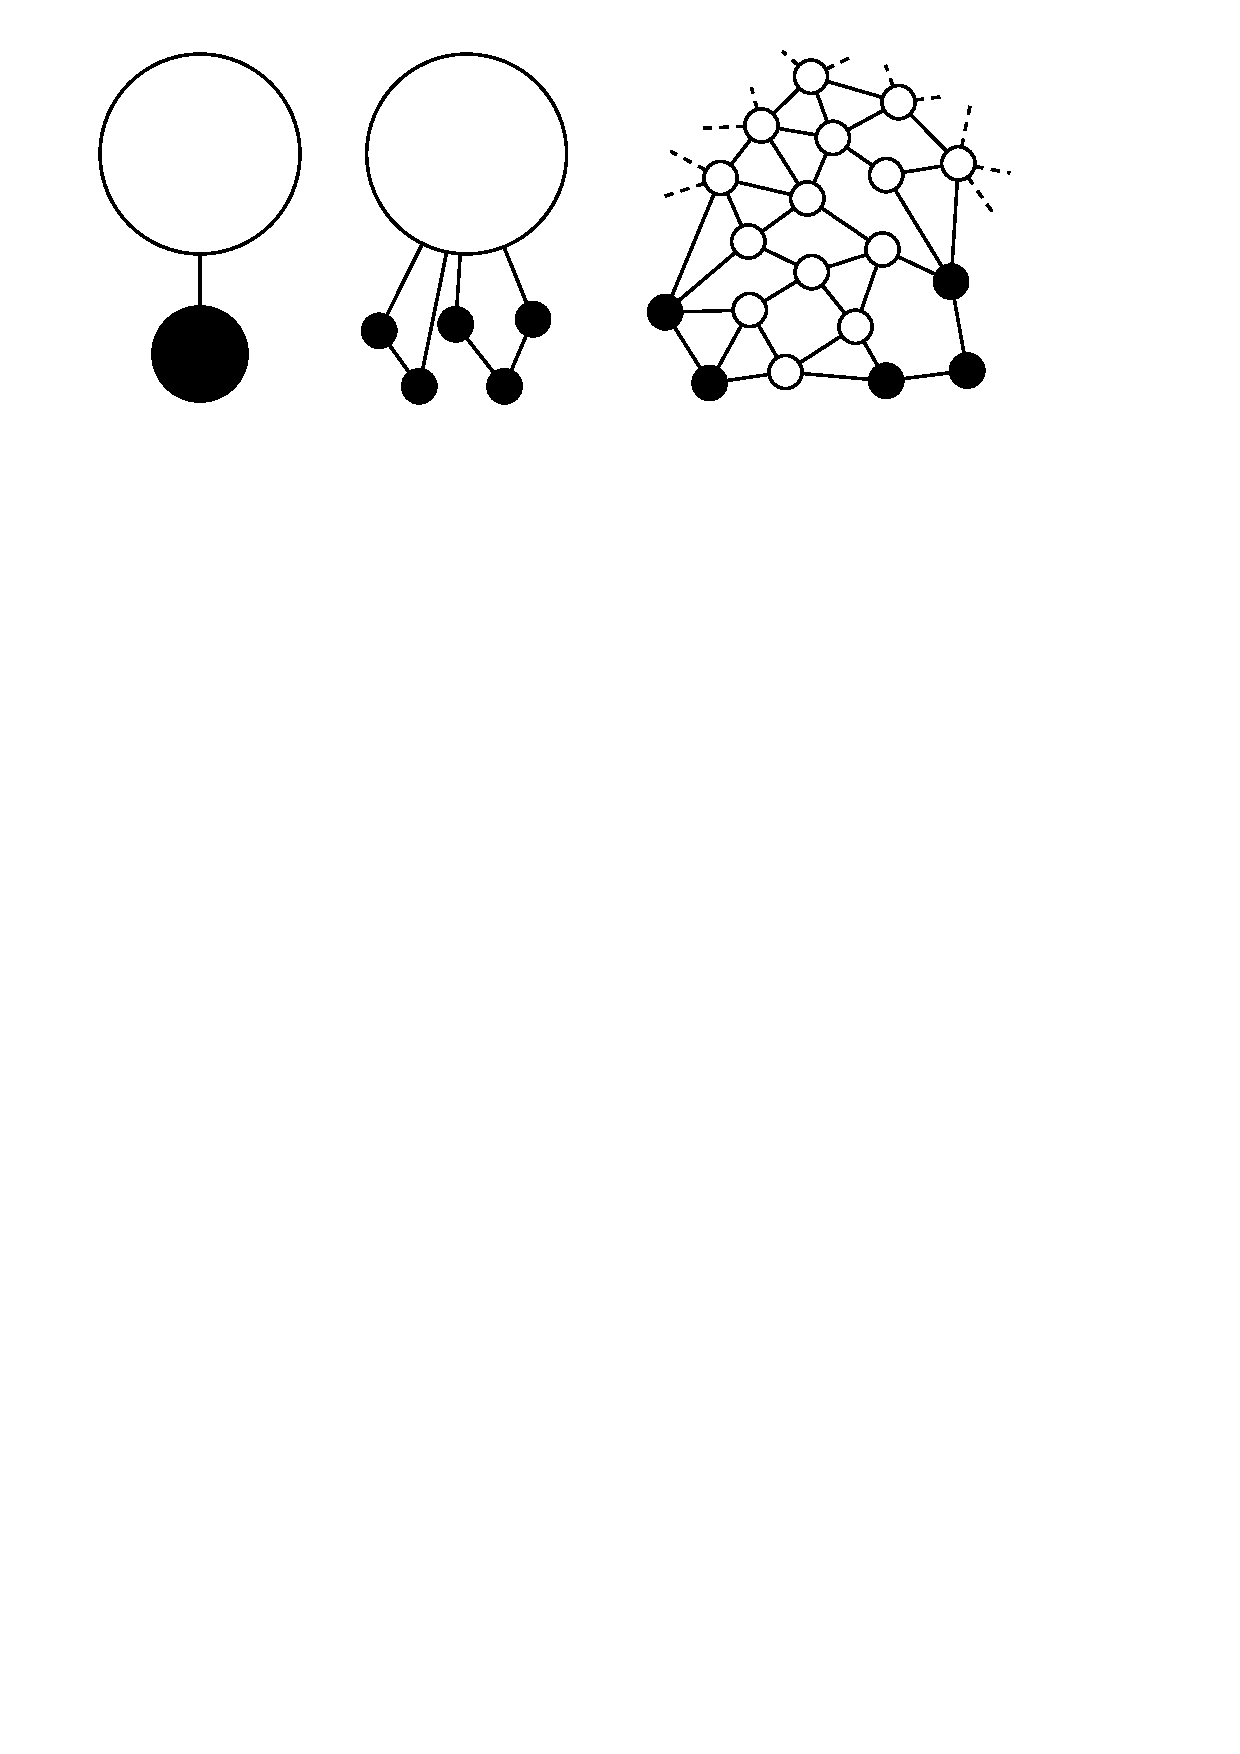
\includegraphics[width=\textwidth]{Pics/uniform_trenn.pdf}
	\caption{Beispielhafter Ablauf der zur Trennung einer Gruppe führt: Durch ungünstige Kantenzusammenhänge und einen entscheidenden Größenunterschied drängt sich die weiße Gruppe zwischen die Knoten der schwarzen Gruppe.}
	\label{Uniform-Trenn-Skizze}
\end{center}
\end{figure}


\paragraph*{Änderungskonstanz}
Durch die unabhängigen internen und externen Gruppenlayouts bei KBK und HL, sind die Änderungen beim Öffnen und Schließen von Gruppen eher gering: Die Layouts in den Gruppen ist unabhängig davon ob andere Gruppen geöffnet oder geschlossen sind und die relativen Positionen der Gruppen zueinander ändern sich selten.

Da bei UKB die Gruppen nicht \glqq geschirmt \grqq\ sind, ist das Layout geöffneter Gruppen sehr stark vom Zustand anderer Gruppen abhängig. Die relativen Positionen bleiben durch die Anker zwar meist erhalten, aber kleine Gruppen sind durchaus anfällig von großen Gruppen deformiert bzw. verdrängt zu werden.

\paragraph*{Komplexität des Algorithmus}
Wie bereits in Kapitel 3 dargestellt, ist der für KBK nötige Algorithmus recht komplex und enthält einige Parameter, die noch bestimmt werden müssen.

Der für HL benötigt Algorithmus benötigt etwas weniger Komplexität als KBK, da die Port für Kanten stets fest sind, wodurch die Größe von geöffneten Gruppen einmalig \glqq Bottom-Up \grqq\ bestimmt werden kann ohne Approximationen und Korrekturen. Allerdings besitzt der zugrundeliegende Algorithmus für hierarchisches Layouts eine höhere Komplexität als kräftebasierende Verfahren.

Der UKB-Algorithmus stellt schließlich eine algorithmisch weniger komplexe Erweiterung von einfachen kräftebasierten Verfahren dar, was vermutlich zu der geringsten Komplexität unter den hier verglichenen Ansätzen führt.

\paragraph*{Anforderung an Graphen}
Während alle hier vorgestellten Ansätze davon ausgehen, dass jeder Knoten und jede Gruppe maximal einer übergeordneten Gruppe zugehört, werden nur bei HL tatsächliche Anforderungen an die eigentliche Graphenstruktur (Zyklenfreiheit) gestellt um problemlos zu funktionieren.

\paragraph*{Kompaktheit}
Sowohl bei KBK als auch bei HL verliert man durch die Kapselung von Gruppen viel Kompaktheit, da hierbei oft Räume in den Gruppen entstehen, die nicht von anderen Gruppen und Knoten genutzt werden können. Das Gesamtlayout bei KBK ist allerdings bei allen Graphen eher zentriert und rund, da es kräftebasiert bestimmt wird, während HL bei unausgeglichenen Graphen zu besonders hohen bzw. stellenweise sehr breiten Graphen führt.

Das Layout des UKB-Ansatzes führt zu ähnlich kompakten Graphen wie herkömmliche kräftebasierte Algorithmen, da die einzigen zusätzlichen Kräfte, die Anker, an den Positionen der Gruppenknoten gesetzt werden, also in der Hüllkurve des Graphen liegen, und ausschließlich anziehend wirken.

\section*{Fazit}
Wie man an den Einzelpunkten erkennt, vereint der Ansatz für den wir uns entschieden haben viele der positiven Eigenschaften der beiden anderen Ansätze bzw. stellt einen Kompromiss zwischen den beiden dar.
%\todo[inline]{Allgemeine Auswertung des Ansatzes/Verfahren schreiben?}
% gesammelte Argumente
	% KB alles kräftebasiert, HS hierarchisch/''Stufen''-Layout
% + Gruppen vorallem semantisch organisiert, weniger strukturell als bei KB
% + Änderungskonstanz der Gruppen (innerhalb von Gruppe) als bei KB
% - komplexer als KB
% + Gruppen überschneiden sich nicht wie bzw einfach zu getrennt zu halten als bei KB 
% + HS ist nur ohne Zykel gut umsetzbar
% + komptakter als HS
% - Struktur evtl nicht so sichtbar wie bei HS aber auch wie bei KB
% + iterativ anwendbar
% + schöner :)
% o Gruppen im Vordergrund der Darstellung durch Ports, nicht Knoten
% o Kantenrounting nicht unbedingt trivial
% 


\chapter{Zusammenfassung und Ausblick}
\label{ch:zsf}

In dieser Arbeit haben wir uns mit dem Layoutproblem für Argumentkarten, welche vordefinierte Gruppenzugehörigkeiten enthalten, beschäftigt. Besonderer Fokus wurde außerdem darauf gelegt, dass die entsprechenden Gruppen vollständig oder komprimiert dargestellt werden können. 

%In dieser Arbeit haben wir mit dem Layoutproblem für Argumentkarten beschäftigt, insbesondere bezüglich vordefinierten Gruppen von Argumenten, d.h. Gruppenzugehörigkeiten sind ein Teil des zu zeichnenden Graphen im Gegensatz zu Gruppen, die als Teil des Layouts bestimmt werden (wie bspw. Graph-Clustering).
\todo[inline]{1. Abschnitt unklar -- jetzt klar?}
\todo[inline]{Graph-Clustering in die Einleitung verschieben/kopieren -- welches von beidem machen wir?}

Unser Lösungsansatz beschreibt eine Konstruktion, die aufbauend auf gebräuchlichen kräftebasierte Algorithmen, Layouts erstellt, die vordefinierte Gruppen herausstellen. Zusätzlich erlaubt der vorgestellte Ansatz das Anzeigen von Gruppen in geöffneten oder geschlossenen Zuständen. Besonderer Fokus wurde zusätzlich auf das Ästhetikkriterium gelegt, dass das Layout sich durch Öffnen und Schließen der Gruppen nur gering verändert.

Eine konkrete Implementierung und entsprechende Auswertung wurde in dieser Arbeit nicht durchgeführt.
Bei einer groben Abschätzung scheint unser Algorithmus keine Operation zu beinhalten, die asymptotisch aufwändiger ist als die quadratische Laufzeit eines gewöhnlichen kräftebasierenden Algorithmus.
%\todo[inline]{Citation needed?}

Zukünftige Arbeiten können sich mit der in dieser Arbeit unterlassenen Implementation und Auswertung beschäftigen. Ein Teil einer solchen Implementierung sollte es sein, die Parameter, welche bei der Beschreibung des Algorithmus bewusste nicht festgelegt wurden, konkret abzuschätzen.
% Außerdem Vorschläge: Öfters hoch und runter bei Layoutberechnung. Ports nicht ganz fest. Kanten abrunden

Alternativ sind auch Ausarbeitungen und Untersuchungen der alternativen Ansätze, die diese Arbeit nur grob umrissen hat, möglich.



%\section{Quellen}
\bibliography{SeminarAlgoQuellen}

\chapter*{About}
Entstanden im Rahmen des Seminars Visualisierung komplexer Argumentation bzw. Algorithmen zur Visualisierung von Debatten 
am Karlsruher Institut für Technology im Wintersemester 2014-15 unter der Leitung von 
Jun.-Prof. Gregor Betz, Diplom Inform. Andreas Gemsa und Dr. Ignaz Rutter.


\end{document}




